% ============================================================================
%  Курсовая работа магистра 1 курса ВМК МГУ
%  Тема: «Оптимизация обновления электрофоретического дисплея»
%  Компилируется через XeLaTeX (для нормальной кириллицы и fontspec).
%  Сборка: `make build` (см. Makefile) или
%          xelatex -interaction=nonstopmode -output-directory=dist thesis.tex
%          biber -output-directory dist dist/thesis
%          xelatex -interaction=nonstopmode -output-directory=dist thesis.tex
%          xelatex -interaction=nonstopmode -output-directory=dist thesis.tex
% ============================================================================

\documentclass[14pt,a4paper,oneside]{extreport}

% ---- 1. Кодировки, языки, шрифты ------------------------------------------
\usepackage{fontspec}
\setmainfont{Times New Roman}
\setsansfont{Arial}
% PT Mono — отечественный моноширинный шрифт с полной кириллической поддержкой,
% поставляется с macOS «из коробки». На Linux обычно есть в пакете fonts-paratype;
% на Windows — fallback на Consolas через \newfontfamily{\cyrillicfonttt}{Consolas}.
\setmonofont{PT Mono}[Scale=0.95]
\newfontfamily{\cyrillicfonttt}{PT Mono}[Scale=0.95]

\usepackage{polyglossia}
\setdefaultlanguage{russian}
\setotherlanguage{english}

% ---- 2. Геометрия страницы (ГОСТ 7.32-2017: 30/15/20/20 мм) ---------------
\usepackage[a4paper,
            left=30mm, right=15mm,
            top=20mm, bottom=20mm,
            footskip=10mm]{geometry}

% Полуторный интервал
\usepackage{setspace}
\onehalfspacing

% Чуть мягче переносы для русского, иначе длинные слова уходят за поля.
\sloppy
\hbadness=10000
\hfuzz=8pt
\tolerance=2000
\emergencystretch=2em

% Абзацный отступ — 1.25 см, без вертикальных пропусков между абзацами
\usepackage{indentfirst}
\setlength{\parindent}{1.25cm}
\setlength{\parskip}{0pt}

% ---- 3. Математика ---------------------------------------------------------
\usepackage{amsmath,amssymb,amsthm,mathtools}
\usepackage{bm}

% Теоремные окружения (по ГОСТ — сквозная нумерация по главам)
\theoremstyle{plain}
\newtheorem{theorem}{Теорема}[chapter]
\newtheorem{lemma}[theorem]{Лемма}
\newtheorem{corollary}[theorem]{Следствие}
\newtheorem{proposition}[theorem]{Утверждение}

\theoremstyle{definition}
\newtheorem{definition}{Определение}[chapter]
\newtheorem{example}{Пример}[chapter]
\newtheorem{remark}{Замечание}[chapter]

\renewcommand{\proofname}{Доказательство}

% ---- 4. Графика, таблицы, плавающие объекты -------------------------------
\usepackage{graphicx}
\graphicspath{{figures/}{figures/diagrams/}{figures/plots/}{figures/raw_photos/}{figures/screenshots/}}

\usepackage{float}
\usepackage{caption}
% ГОСТ: подпись "Рисунок N — Название" под рисунком, "Таблица N — Название" над таблицей
\captionsetup[figure]{name=Рисунок,labelsep=endash,format=plain,justification=centering,singlelinecheck=false}
\captionsetup[table]{name=Таблица,labelsep=endash,format=plain,justification=raggedright,singlelinecheck=false,position=above}

\usepackage{booktabs}
\usepackage{array}
\usepackage{longtable}
\usepackage{multirow}
\usepackage{tabularx}      % таблицы с авто-шириной колонок
\usepackage{placeins}      % \FloatBarrier для жёсткого размещения figures

% Float-параметры: разрешаем больше материала на странице, чтобы
% избежать pile-up'а из-за слишком ограниченных дефолтов LaTeX.
\renewcommand{\topfraction}{0.85}
\renewcommand{\bottomfraction}{0.7}
\renewcommand{\textfraction}{0.15}
\renewcommand{\floatpagefraction}{0.7}
\setcounter{topnumber}{4}
\setcounter{bottomnumber}{4}
\setcounter{totalnumber}{6}
\usepackage{tikz}          % векторные диаграммы прямо в .tex
\usetikzlibrary{positioning, arrows.meta, decorations.pathreplacing, calc, shapes.geometric, patterns}

% ---- 5. Листинги кода ------------------------------------------------------
\usepackage{listings}
\lstset{
    basicstyle=\ttfamily\small,
    breaklines=true,
    columns=fullflexible,
    frame=single,
    numbers=left,
    numberstyle=\tiny\color{gray!60},
    keywordstyle=\color{blue!70!black},
    commentstyle=\color{green!50!black}\itshape,
    stringstyle=\color{red!60!black},
    showstringspaces=false,
    captionpos=b,
}
\renewcommand{\lstlistingname}{Листинг}

\usepackage{xcolor}

% ---- 6. Гиперссылки --------------------------------------------------------
\usepackage[unicode]{hyperref}
\hypersetup{
    colorlinks=true,
    linkcolor=black,        % внутренние ссылки чёрные (по ГОСТу)
    citecolor=black,
    urlcolor=blue!50!black,
    pdftitle={Оптимизация обновления электрофоретического дисплея},
    pdfauthor={Ахроян Г. (ВМК МГУ)},
    pdflang={ru-RU},
}

% ---- 7. Библиография (ГОСТ Р 7.0.5-2008 через biblatex-gost) --------------
\usepackage[backend=biber,
            style=gost-numeric,
            sorting=none,
            language=auto,
            autolang=other,
            babel=other,
            maxbibnames=10,
            minbibnames=10]{biblatex}
\addbibresource{bib/bibliography.bib}

% ---- 8. Заголовки разделов (ГОСТ-стиль) ------------------------------------
\usepackage{titlesec}
% Глава: 14pt, по центру, прописные, жирный
\titleformat{\chapter}[block]
  {\normalfont\large\bfseries\centering}
  {\thechapter}{1em}{\MakeUppercase}
\titlespacing*{\chapter}{0pt}{0pt}{1.5em}

% Section: 14pt, слева, обычный регистр
\titleformat{\section}[block]
  {\normalfont\normalsize\bfseries}
  {\thesection}{1em}{}
\titlespacing*{\section}{0pt}{1em}{0.5em}

\titleformat{\subsection}[block]
  {\normalfont\normalsize\bfseries\itshape}
  {\thesubsection}{1em}{}
\titlespacing*{\subsection}{0pt}{0.5em}{0.25em}

% ---- 9. Оглавление --------------------------------------------------------
\renewcommand{\contentsname}{Оглавление}
\usepackage{tocloft}

% ---- 10. Прочее ------------------------------------------------------------
\usepackage{enumitem}
% nosep — без вертикальных промежутков между пунктами.
% leftmargin=\parindent выравнивает левый край маркера с абзацным отступом
% основного текста (1.25см), чтобы списки визуально не торчали к левому полю.
\setlist{nosep,leftmargin=\parindent,itemindent=0pt,labelsep=0.5em}

\usepackage{microtype}

% Команда для подписи рисунка по ГОСТ (если нужна вручную)
\newcommand{\gostfigure}[3]{%
    \begin{figure}[H]
        \centering
        \includegraphics[width=#2]{#1}
        \caption{#3}\label{fig:#1}
    \end{figure}
}

% ============================================================================
%                                ДОКУМЕНТ
% ============================================================================

\begin{document}

% --- Титульный лист ---
% Титульный лист (ГОСТ 7.32-2017, форма для ВМК МГУ)
\thispagestyle{empty}

\begin{center}
    \fontsize{12pt}{14pt}\selectfont

    \uppercase{Министерство науки и высшего образования}\\
    \uppercase{Российской Федерации}

    \vspace{0.5em}

    Федеральное государственное бюджетное образовательное\\
    учреждение высшего образования\\
    \textbf{«МОСКОВСКИЙ ГОСУДАРСТВЕННЫЙ УНИВЕРСИТЕТ}\\
    \textbf{имени М.\,В. Ломоносова»}

    \vspace{0.5em}

    \uppercase{Факультет вычислительной математики и кибернетики}

    \vspace{0.3em}

    Кафедра \rule{6cm}{0.4pt}
    % TODO: указать кафедру

    \vfill

    {\fontsize{16pt}{20pt}\selectfont\bfseries
        КУРСОВАЯ РАБОТА\\
        магистра 1 курса
    }

    \vspace{2em}

    {\fontsize{16pt}{20pt}\selectfont\bfseries
        «Оптимизация обновления\\
        электрофоретического дисплея»
    }

    \vfill

\end{center}

\begin{flushright}
    \fontsize{12pt}{16pt}\selectfont

    \textbf{Выполнил:}\\
    студент \rule{5cm}{0.4pt}\\
    Ахроян Г. % TODO: уточнить группу и полное ФИО

    \vspace{1.5em}

    \textbf{Научный руководитель:}\\
    \rule{6cm}{0.4pt}\\
    % TODO: ФИО, степень, должность научного руководителя
\end{flushright}

\vfill

\begin{center}
    \fontsize{12pt}{14pt}\selectfont
    Москва, 2026
\end{center}

\clearpage


% --- Оглавление ---
\tableofcontents
\clearpage

% --- Основные главы ---
\chapter{Введение}\label{ch:intro}

% TODO (M2): Развёрнутое введение.
% Структура (по Chapter Plan, RESEARCH.md → § 1, ~3 страницы):
%   1.1 Актуальность темы
%       — массовое применение EPD (e-readers, ценники, signage);
%       — конфликт «энергия ↔ ghosting ↔ скорость ↔ ресурс»;
%       — состояние области (Kang 2025, Lai 2026 — современные алгоритмы);
%       — пробел: нет работ со структурной теоремой об оптимальной форме waveform.
%   1.2 Цель и задачи работы
%   1.3 Научная новизна
%       — N2+N1 гибрид: алгоритм + структурная теорема (bang-bang с ≤K_eff фаз);
%       — каскадная теория PDE → ODE → дискретный PMP → Парето;
%       — экспериментальная валидация на стенде.
%   1.4 Положения, выносимые на защиту (3-4 пункта)
%   1.5 Апробация (если будет — конференция / препринт)
%   1.6 Структура работы

\section*{Заглушка}

Раздел будет наполнен на этапе~M2 в соответствии с Chapter Plan
(см. \texttt{.ai-factory/RESEARCH.md}).

Тест цитирования (будет удалён на~M2): современные обзоры предметной
области~\cite{zhong2026_review,heikenfeld2011_review}, базовая физика
электрофореза~\cite{comiskey1998_nature,yang2021_mechanisms}, прямые
конкуренты по waveform-оптимизации~\cite{kang2025_dp_waveform,lai2026_e3dw_energy}.
Используемая математическая база~\cite{pontryagin1983_optimal_processes,vasiliev2002_methods,phogat2017_discrete_pmp}.

\chapter{Обзор предметной области}\label{ch:review}

\section{Архитектура электрофоретического дисплея}\label{sec:epd-arch}

Электрофоретический дисплей (Electrophoretic Display, EPD) --- отражательное
устройство визуализации, изображение в котором формируется позиционированием
заряженных пигментных частиц внутри микрокапсул, заполненных непроводящей
жидкостью. Технология введена Comiskey~и~соавторами в 1998~году~\cite{comiskey1998_nature},
впервые продемонстрировавшими изготовление отражательного дисплея методами
печатной технологии. С тех пор EPD заняли устойчивую нишу в продуктах,
требующих низкого среднего энергопотребления и читаемости при внешнем
освещении: ридерах электронных книг (Amazon~Kindle, Kobo, ONYX~BOOX),
электронных ценниках, низкоэнергетических индикаторах для интернета вещей и
носимой электроники.

Принцип работы микрокапсулы основан на электрофоретическом смещении двух типов
частиц с противоположными знаками заряда (обычно белых частиц диоксида
титана~$\mathrm{TiO}_2$ и чёрных частиц технического углерода) под действием
поля на электродах пикселя~\cite{yang2021_mechanisms}. В активных матрицах
(active matrix EPD, AM\nobreakdash-EPD) индивидуальное управление нижними
электродами реализуется тонкоплёночными транзисторами; общая структура
устройства показана на рисунке~\ref{fig:02_am_epd_arch}.

\begin{figure}[H]
    \centering
    \begin{tikzpicture}[font=\small, scale=1.0]
        % Верхний прозрачный ITO электрод
        \draw[fill=cyan!10, draw=cyan!60!black, thick]
            (0, 2) rectangle (9, 2.4);
        \node[right=0.1cm] at (9, 2.2) {ITO common electrode};

        % Слой микрокапсул (3 капсулы)
        \foreach \x in {1.5, 4.5, 7.5} {
            \draw[fill=gray!5, draw=gray!50, thick] (\x, 1) circle (1.0);
        }

        % Частицы внутри: белые сверху, чёрные снизу
        \foreach \x in {1.5, 4.5, 7.5} {
            % белые частицы (T iO2) — наверху
            \foreach \y/\xx in {1.6/0, 1.7/0.3, 1.5/-0.4, 1.6/-0.2} {
                \draw[fill=white, draw=black, thin] (\x+\xx, \y) circle (0.10);
            }
            % чёрные частицы — внизу
            \foreach \y/\xx in {0.6/0.1, 0.55/-0.3, 0.65/-0.05, 0.5/0.35} {
                \draw[fill=black] (\x+\xx, \y) circle (0.10);
            }
        }

        % Нижний электрод (TFT матрица — сегментированный)
        \foreach \x in {0, 1.5, 3, 4.5, 6, 7.5} {
            \draw[fill=yellow!20, draw=brown, thick]
                (\x+0.1, -0.3) rectangle (\x+1.4, 0);
        }
        \node[below=0.1cm] at (4.5, -0.3) {TFT-подложка (сегментированная)};

        % Управляющее напряжение
        \draw[<->, thick, gray] (-0.5, 0) -- (-0.5, 2.4)
            node[midway, left] {\rotatebox{90}{$U(t)$}};

        % Метки сторон
        \node[above right] at (0, 2.4) {\small (+)};
        \node[below right] at (0, -0.3) {\small (--)};
    \end{tikzpicture}
    \caption{Архитектура активно-матричного электрофоретического дисплея.
        Сверху --- общий прозрачный ITO электрод, снизу --- сегментированная
        TFT-матрица (подложка). Между электродами --- слой микрокапсул с
        белыми (TiO$_2$) и чёрными частицами противоположных зарядов.
        Управляющее напряжение $U(t)$ задаёт направление электрофоретического
        смещения частиц и тем самым видимое оптическое состояние пикселя.}
    \label{fig:02_am_epd_arch}
\end{figure}
\FloatBarrier

Ключевое физическое свойство EPD --- \emph{бистабильность}: после снятия
управляющего поля частицы сохраняют положение часами и днями без
энергопотребления~\cite{yang2021_mechanisms}. Это отличает EPD от
жидкокристаллических и органических светодиодных дисплеев, где поддержание
изображения требует непрерывного тока. За счёт бистабильности в статическом режиме
энергопотребление близко к нулю, а заметные затраты приходятся только на момент
обновления.

С точки зрения моделирования EPD относятся к классу
электрофоретико-диэлектрофоретических систем. Помимо силы
электрофореза~$\vec{F}_{\!\text{EP}} = q \vec{E}$ на заряженную частицу, в
неоднородном поле существенна сила диэлектрофореза
$\vec{F}_{\!\text{DEP}} \propto \nabla |\vec{E}|^2$, объясняющая отклик пикселей
на переменное поле и эффективный порог переключения при пассивной
адресации~\cite{bert2003_physics}. В рассматриваемом здесь режиме
(последовательность постоянных импульсов с обнулённым средним зарядом) вкладом
DEP можно пренебречь, что обсуждается в главе~\ref{ch:model}.


\section{Таксономия методов проектирования waveform}\label{sec:taxonomy}

Под \emph{waveform} в EPD понимается последовательность дискретных фаз
$(V_k, T_k)_{k=1}^{K}$, прикладываемых к пикселю при переходе между уровнями
серого. Её конфигурация --- основной (и обычно единственный программно
доступный) инструмент оптимизации обновления EPD на уровне контроллера.
Накопленный за два десятилетия пул работ систематизирован в
обзоре~\cite{zhong2026_review}; на его основе ниже выделены пять
направлений, наиболее значимых для постановки настоящей работы.

\subsection*{Исторический фундамент}

Базовая трёхстадийная структура waveform (\emph{erase} — \emph{activate} —
\emph{drive}) предложена Zehner~и~соавторами в 2003~году (цитируется
по~\cite{kang2025_dp_waveform}). Все последующие модификации waveform для
b/w-панелей сохраняют эту трёхчастную базу, варьируя структуру отдельных стадий.

\subsection*{Подавление ghosting}

Wang~и~соавторы~\cite{wang2022_red_ghost} снизили «красный гостинг» в
трёхцветных EPD, разделив этап стирания на две части (специализированную для
красных частиц и стандартную) и применив высокочастотный прямоугольный сигнал
на этапе активации. Подавление остаточного изображения составило 80{,}43\,\%,
интенсивности фликера — 79{,}63\,\%. Авторы отдельно оговаривают
требование нулевого суммарного заряда (DC balance compliance),
вытекающее из физики накопления заряда в микрокапсуле и подтверждаемое
сокращением ресурса панели при несбалансированных
waveform~\cite{yang2021_mechanisms}.

\subsection*{Ускорение отклика}

He~и~соавторы~\cite{he2020_particle_activation} разделили активационную фазу на
две подфазы: повышение подвижности частиц и установление референсного уровня
серого. Длительность первой подфазы выбирается по точке перегиба эмпирической
кривой яркости (момент максимума скорости частиц). На панели~ED060SC7 это
сократило полное время обновления на~300\,мс при подавлении гостинга на~57\,\%
и снижении фликера на~26{,}7\,\%.

\subsection*{Снижение энергопотребления}

Наиболее свежие работы по энергоэффективности --- Lin~и~соавторов~\cite{lin2024_low_power}
и Lai~и~соавторов~\cite{lai2026_e3dw_energy}.

Lin~и~соавторы исходят из соотношения для пиковой мощности обновления:
\begin{equation}\label{eq:p-peak}
    P_{\text{peak}} \;=\; \tfrac{1}{2}\,C\,\Delta V^{2}\, f\, V_{\text{source}},
\end{equation}
где $C$~--- эквивалентная ёмкость пикселя, $\Delta V$~--- амплитуда скачка
напряжения между соседними фазами, $f$~--- частота переключений,
$V_{\text{source}}$~--- максимальное напряжение источника.\footnote{Соотношение
приводится в записи первоисточника~\cite{lin2024_low_power}; размерно оно
отвечает мощности с точностью до множителя $V_{\text{source}}$ и используется
авторами как качественный индикатор зависимости потребления от $\Delta V$ и
$f$. В собственной энергетической модели настоящей работы (гл.~\ref{ch:experiment})
применяется калибровка на уровне панели, а не эта формула.} Уменьшение числа
смен полярности и нулевые вставки в waveform снизили энергетическую флуктуацию
на~37{,}24\,\% и среднюю мощность на тестовом наборе из девяти изображений.

Lai~и~соавторы предлагают системно-уровневое решение E3DW
(\emph{Energy-Efficient E-Paper Driving Waveform}), объединяющее анализ
содержимого кадра, компенсацию по температуре и низкочастотный прямоугольный
сигнал (1--5\,Гц). На цветном EPD достигнуто снижение энергопотребления
на~35{,}7\,\% относительно базовой конфигурации.

\subsection*{Алгоритмическая оптимизация на основе динамического программирования}

Kang~и~соавторы~\cite{kang2025_dp_waveform} представляют наиболее близкий к
настоящей работе подход: строят дискретный граф состояний пикселя и применяют
динамическое программирование для поиска оптимального пути по скаляризованному
критерию --- взвешенной сумме времени отклика, фликера и качества изображения
с весами~$0{,}6$, $0{,}2$ и~$0{,}2$. Главное ограничение (см.~раздел~\ref{sec:gap}) --- фиксация весов: решение есть единственная точка в
пространстве~$(E, G, \tau)$, без исследования компромиссов между целями.

\subsection*{Сравнительная таблица}

В таблице~\ref{tab:waveform-methods} собраны рассмотренные методы с указанием
оптимизируемых величин, алгоритмической основы и заявленных результатов;
в последней строке для сопоставления приведена позиция настоящей работы.

\begin{table}[H]
    \caption{Сравнение современных методов проектирования waveform для EPD}\label{tab:waveform-methods}
    \begin{tabular}{l p{3.5cm} p{3.5cm} p{3.5cm}}
        \toprule
        Источник & Что оптимизируется & Алгоритмическая основа & Результат \\
        \midrule
        Zehner~2003 (cit.\ \cite{kang2025_dp_waveform}) & базовая структура waveform & ручной дизайн & базовая трёхстадийная схема \\
        He~2020~\cite{he2020_particle_activation} & время отклика & эвристика точки перегиба & $-300$\,мс, $-57\,\%$ ghost \\
        Wang~2022~\cite{wang2022_red_ghost} & красный гостинг (3-color) & разделение стадии стирания & $-80{,}4\,\%$ ghost \\
        Lin~2024~\cite{lin2024_low_power} & пиковая мощность & вставки нулевого напряжения & $-37\,\%$ флуктуация энергии \\
        Lai~2026~\cite{lai2026_e3dw_energy} & энерго\-потребление & system-level E3DW & $-35{,}7\,\%$ энергии \\
        Kang~2025~\cite{kang2025_dp_waveform} & скаляризованный $(\tau, G, \text{кач.})$ & динамическое программирование & оптимальный путь, single objective \\
        \textbf{Настоящая работа} & \textbf{Парето-граница $(E, G, \tau)$} & \textbf{$\varepsilon$-constraint + дискретный PMP} & \textbf{весь Парето-фронт, а не одна точка} \\
        \bottomrule
    \end{tabular}
\end{table}


\section{Контроллер SSD1680}\label{sec:ssd1680}

Аппаратной базой работы служит контроллер SSD1680 производства
Solomon~Systech~\cite{ssd1680_datasheet}, управляющий панелью
Waveshare~2.13''~V4. Его архитектура задаёт конечномерную дискретную постановку
задачи оптимального управления, формализуемую в~главе~\ref{ch:theorem}.

\subsection*{Структура waveform setting и регистр 0x32}

Согласно разделу~6.7 datasheet, полный waveform setting состоит из~159 байт,
кодирующих все управляющие параметры одного обновления: 153~байта LUT
(записываются командой~$0x32$) и по одному байту для выходных напряжений
$V_{\text{GH}}$, $V_{\text{SH1}}$, $V_{\text{SH2}}$, $V_{\text{SL}}$,
$V_{\text{COM}}$ плюс опциональный байт окончания процедуры. Структура LUT ---
5 sub-LUT $\times$ 12 фаз $\times$ 4 sub-frame; в каждой ячейке выбирается один
из пяти уровней напряжения
$\{V_{\text{SH1}}, V_{\text{SH2}}, V_{\text{SL}}, V_{\text{COM}}, 0\}$, что
задаёт конечный алфавит управляющих воздействий мощностью~$|U| = 5$.

Для каждой фазы дополнительно указываются длительности обоих sub-frame'ов
$\mathrm{TP}_k^{X}$, параметры наклона переходов~$\mathrm{SR}_k^{XY}$, число
повторений фазы $\mathrm{RP}_k$, частота кадров $\mathrm{FR}_k$ и битовый флаг
gate-gating $\mathrm{XON}_k^{XY}$. В совокупности они задают конечномерное
пространство допустимых waveform с явной структурой управления.

\subsection*{Поиск waveform по температуре в OTP}

Помимо программно-записываемого LUT контроллер хранит во встроенной однократно
программируемой памяти (One-Time Programmable, OTP) до~36 температурно-индексированных
waveform setting (TR0\ldots TR35). Команды $0x18$ (выбор источника датчика
температуры) и $0x22$ с битом «загрузить значение температуры» инициируют поиск
подходящей записи в OTP и её загрузку в регистр~$0x32$~\cite{ssd1680_datasheet}.

\subsection*{Семантика регистра 0x22 и условие применимости пользовательской LUT}

Регистр $0x22$ (\emph{Display Update Control~2}) задаёт последовательность
операций при активации обновления командой~$0x20$. Восемь основных значений и
соответствующие последовательности приведены в
datasheet~\cite{ssd1680_datasheet}; для нас важны четыре варианта:

\begin{itemize}
    \item $0x{}C7$~/~$0x{}CF$ — последовательность \emph{«включить аналоговое
    питание $\to$ запустить обновление в режиме Display Mode 1/2 $\to$ выключить
    аналоговое питание $\to$ выключить генератор»}, использующая waveform,
    \emph{уже записанный пользователем} в регистр~$0x32$;
    \item $0x{}F7$~/~$0x{}FF$ — тот же набор операций с дополнительным шагом
    \emph{«загрузить значение температуры»}, инициирующим Waveform Setting
    Searching Mechanism и перезапись пользовательского LUT заводским вариантом
    из OTP.
\end{itemize}

Отсюда следует, что применение пользовательской waveform-LUT возможно
\emph{исключительно} через значение $0x{}C7$ (полное обновление) или $0x{}CF$
(частичное); использование $0x{}F7$~/~$0x{}FF$ эквивалентно отказу от
пользовательской waveform. Это наблюдение, отсутствующее в reference-реализации
Waveshare~\cite{waveshareteam_epaper}, воспроизведено и подтверждено в
экспериментах работы (см.~раздел~\ref{ch:experiment}). Без указанного фикса
любые алгоритмические улучшения waveform неприменимы на физическом стенде.


\section{Постановка задачи и её отличие от существующих работ}\label{sec:gap}

В рассмотренных в~разделе~\ref{sec:taxonomy} работах отсутствует ряд элементов,
существенных для систематической инженерной оптимизации обновления EPD.

Во-первых, ни в одной из них нет структурного результата о форме
оптимального waveform. Все цитированные методы предлагают алгоритмические
процедуры поиска: ручную настройку~\cite{wang2022_red_ghost}, эвристику точки
перегиба~\cite{he2020_particle_activation}, перебор
конфигураций~\cite{lin2024_low_power} или динамическое
программирование~\cite{kang2025_dp_waveform}. Знание структуры оптимума
(например, что оптимальное управление имеет релейную (bang-bang) структуру с
числом активных фаз, ограниченным размерностью пространства состояний)
позволило бы a~priori сузить пространство поиска и обосновать тип кандидатных
waveform.

Во-вторых, все эти работы оптимизируют одну целевую функцию или
фиксированную скаляризацию нескольких целей: Kang~и~соавторы~\cite{kang2025_dp_waveform}
--- веса $(0{,}6;\, 0{,}2;\, 0{,}2)$; \cite{lin2024_low_power} --- только
пиковую мощность; \cite{lai2026_e3dw_energy} --- суммарную энергию. При этом
авторы обзора~\cite{zhong2026_review} отмечают, что в реальных приложениях вес
каждой цели сильно зависит от сценария: для мобильных устройств критична
энергия, для считывающих --- латентность, для систем длительного отображения
--- гостинг. Единственной точки в пространстве $(E, G, \tau)$ недостаточно для
осмысленного адаптивного выбора waveform.

В-третьих, управляющие ограничения нигде не выводятся из
физико-математической модели устройства. Прежде всего это касается условия
нулевого суммарного заряда, \emph{зарядового баланса}. Оно упоминается как общепринятая
практика~\cite{wang2022_red_ghost, yang2021_mechanisms}, но не интегрируется в
формальную постановку оптимизационной задачи.

Наконец, валидация в~\cite{kang2025_dp_waveform,
lai2026_e3dw_energy} проводилась на специализированном оборудовании
(колориметры, лабораторные анализаторы мощности), что затрудняет независимое
воспроизведение и сопоставление методик.

Перечисленные пробелы и закрывает настоящая работа: каскадной моделью
обновления (глава~\ref{ch:model}), структурной теоремой о форме оптимума в классе
сбалансированных по заряду waveform (глава~\ref{ch:theorem}), алгоритмом
построения Парето-границы по $(E, G, \tau)$ на базе $\varepsilon$-constraint
метода (глава~\ref{ch:algorithm}) и экспериментальной валидацией на стенде из
общедоступных компонентов с открытым ПО (глава~\ref{ch:experiment}).

\chapter{Физическая модель и редукция}\label{ch:model}

В главе строится модель обновления электрофоретического дисплея на трёх
уровнях абстракции: континуальном (уравнения Пуассона--Нернста--Планка),
усреднённом (система ОДУ для одного пикселя) и дискретном (готовом к
интеграции с задачей оптимального управления гл.~\ref{ch:theorem}). Каждый из
переходов мы сопровождаем допущениями, на которых он держится.
Глава завершается калибровкой эффективных параметров по данным
стенда (гл.~\ref{ch:experiment}).

\section{Микрокапсула и электрофорез}\label{sec:model-capsule}

Базовая структурная единица активной матрицы~--- \emph{микрокапсула}:
сферическая оболочка диаметром $d_{\mathrm{caps}}\sim 40\ldots 50$~мкм,
заполненная непроводящей жидкостью (углеводородная смесь с относительной
проницаемостью $\varepsilon_m \approx 2$). В ней диспергированы пигментные
частицы двух типов: белые (диоксид титана $\mathrm{TiO}_2$) и чёрные
(углеродная сажа) радиусом $R \sim 100\ldots 500$~нм
\cite{comiskey1998_nature, yang2021_mechanisms}. Заряд сообщают агенты
управления зарядом (\emph{charge controlling agents}, CCA)~--- ПАВ,
обменивающие заряды с поверхностью пигмента; при типичной концентрации CCA
заряд частицы~$q$ постоянен на временах одного
обновления~\cite{yang2021_mechanisms}.

Сверху и снизу к капсуле примыкают электроды: общий прозрачный из оксида
индия-олова и сегментированный нижний электрод TFT-матрицы. Напряжение
$U$ создаёт в жидкости поле, смещающее заряженные частицы вдоль
межэлектродной оси и формирующее изображение; смена знака $U$ переключает
оптическое состояние пикселя между «белым» и «чёрным» в зависимости от того,
какие частицы оказываются у верхнего электрода.

\begin{figure}[H]
    \centering
    \begin{tikzpicture}[font=\small, scale=1.0]
        % Внешний контур микрокапсулы (круг)
        \draw[fill=blue!5, draw=blue!50!black, thick] (0, 0) circle (3);
        \node[above=0.1cm] at (0, 3) {Микрокапсула, $d_{\mathrm{caps}} \approx 40$~мкм};

        % Верхний и нижний электроды (касательные плоскости)
        \draw[ultra thick, cyan!60!black] (-3.2, 2.5) -- (3.2, 2.5);
        \node[right=0.1cm] at (3.2, 2.5) {ITO (+)};
        \draw[ultra thick, brown] (-3.2, -2.5) -- (3.2, -2.5);
        \node[right=0.1cm] at (3.2, -2.5) {TFT (--)};

        % Белые частицы (TiO2) — внутри, разбросаны
        \foreach \x/\y in {-1.5/1.5, -0.8/1.0, 0.6/1.7, 1.5/1.2, -0.5/0.5, 1.1/0.3, 0.0/-0.4, -1.7/-0.6, 1.7/-1.2, 0.3/-1.5} {
            \draw[fill=white, draw=black] (\x, \y) circle (0.18);
            \node[font=\tiny] at (\x, \y) {$+$};
        }

        % Чёрные частицы
        \foreach \x/\y in {-1.0/-1.5, 0.8/-1.7, 1.3/0.8, -1.8/0.8, 0.5/0.8, -0.2/1.4, 1.0/-0.9} {
            \draw[fill=black] (\x, \y) circle (0.18);
            \node[font=\tiny, color=white] at (\x, \y) {$-$};
        }

        % Стрелки сил
        \draw[->, very thick, red!70!black] (-2.5, 0) -- (-2.5, 1.5);
        \node[left] at (-2.5, 0.75) {$\vec{F}_E = q\vec{E}$};

        \draw[->, thick, blue!70!black] (2.5, 0.8) -- (2.5, -0.2);
        \node[right] at (2.5, 0.3) {$\vec{F}_{\!\text{Stokes}}$};

        % Поле E
        \node[font=\large] at (0, 2.1) {$\vec{E} \downarrow$};
    \end{tikzpicture}
    \caption{Сферическая микрокапсула электрофоретического дисплея с двумя
        типами заряженных пигментных частиц (белые $\mathrm{TiO}_2$ ---
        положительно заряженные, чёрные углеродные --- отрицательно
        заряженные). Под действием электрического поля $\vec{E}$ на частицу
        действуют электрическая сила $\vec{F}_E = q\vec{E}$ и противоположно
        направленная сила сопротивления среды по закону Стокса
        $\vec{F}_{\!\text{Stokes}} = -6\pi\eta R \vec{v}$.}
    \label{fig:model-capsule}
\end{figure}

Движение частицы определяется балансом электрической силы
$\vec{F}_E = q\vec{E}$ и стоксова сопротивления среды
$\vec{F}_{\mathrm{drag}} = -6\pi\eta R\, \vec{v}$ ($\eta$ — вязкость, $\vec{v}$ —
скорость). В установившемся режиме силы уравновешиваются:
$\vec{v} = q\vec{E}/(6\pi\eta R)$. Время выхода на режим задаёт постоянная
$\tau_{\mathrm{Stokes}} = m/(6\pi\eta R)$ ($m$ — масса частицы), при типовых
параметрах~--- единицы миллисекунд.

В неоднородном поле добавляется диэлектрофоретический вклад
$\vec{F}_{\mathrm{DEP}} = 2\pi r^3 \varepsilon_m\, \operatorname{Re}(K^*) \nabla|\vec{E}|^2$,
существенный для систем с пассивной адресацией без выраженного порога
переключения \cite{bert2003_physics}. В режиме настоящей работы
(последовательность постоянных по знаку импульсов в пределах одной фазы
waveform с обнулённым суммарным зарядом за обновление) им можно пренебречь;
это допущение разбирается в~\ref{sec:model-pde}, а его правомерность подтверждает
согласие упрощённой модели с измерениями (гл.~\ref{ch:experiment}).


\section{Уравнения Пуассона--Нернста--Планка}\label{sec:model-pde}

Континуальное описание концентраций двух типов частиц $c_\pm(x, t)$ строится
на законе сохранения числа частиц, конститутивном соотношении
для потока (сумма диффузионного и дрейфового слагаемых) и уравнении Пуассона,
связывающем распределение заряда с потенциалом.

\subsection*{Уравнение непрерывности}

Из закона сохранения числа частиц типа $\pm$ для произвольного объёма
$\Omega \subset \mathbb{R}^3$ имеем:
\begin{equation}\label{eq:continuity-integral}
    \frac{\partial}{\partial t} \int_{\Omega} c_\pm \, dV
    = -\oint_{\partial \Omega} \vec{J}_\pm \cdot \hat{n}\, dS,
\end{equation}
где $\vec{J}_\pm$ — поток частиц (число частиц через единицу площади в единицу
времени), $\hat{n}$ — внешняя нормаль к $\partial\Omega$. По теореме
Гаусса--Остроградского и в силу произвольности $\Omega$~--- локальная
форма:
\begin{equation}\label{eq:continuity}
    \frac{\partial c_\pm}{\partial t} + \nabla \cdot \vec{J}_\pm = 0.
\end{equation}
Уравнение~\eqref{eq:continuity} не зависит от природы потока; конкретизация
модели — в определении $\vec{J}_\pm$.

\subsection*{Конститутивное соотношение для потока}

При двух движущих силах — градиенте концентрации (диффузия) и
электрическом поле (электрофорез) — поток представим суммой:
\begin{equation}\label{eq:flux}
    \vec{J}_\pm = -D_\pm \nabla c_\pm + c_\pm \vec{v}_\pm,
\end{equation}
где первое слагаемое — закон Фика с коэффициентом $D_\pm$, второе —
конвективный перенос со средней дрейфовой скоростью $\vec{v}_\pm$.

\subsection*{Стоксова дрейфовая скорость}

Для шарообразной частицы радиуса $R_\pm$ с зарядом $q_\pm$ в жидкости вязкости
$\eta$ под действием поля $\vec{E}$ уравнение движения имеет вид:
\begin{equation}\label{eq:newton}
    m_\pm \frac{d\vec{v}_\pm}{dt}
    = q_\pm \vec{E} - 6\pi \eta R_\pm \, \vec{v}_\pm.
\end{equation}
В установившемся режиме ($d\vec{v}_\pm / dt = 0$) баланс сил даёт:
\begin{equation}\label{eq:drift-velocity}
    \vec{v}_\pm = \frac{q_\pm \vec{E}}{6\pi \eta R_\pm}
    \equiv \mu_{e,\pm}\, \vec{E},
    \qquad
    \mu_{e,\pm} \equiv \frac{|q_\pm|}{6\pi \eta R_\pm},
\end{equation}
где $\mu_{e,\pm}$ — \emph{электрофоретическая подвижность}. Знак $q_\pm$ задаёт
направление дрейфа: положительные частицы движутся вдоль поля, отрицательные —
против.

Характерное время релаксации скорости к~\eqref{eq:drift-velocity}
определяется уравнением~\eqref{eq:newton}:
\begin{equation}\label{eq:tau-stokes}
    \tau_{\mathrm{Stokes}} = \frac{m_\pm}{6\pi \eta R_\pm}.
\end{equation}
При типовых параметрах ($m \sim 10^{-17}$~кг, $R \sim 200$~нм,
$\eta \sim 10^{-3}$~Па$\cdot$с) $\tau_{\mathrm{Stokes}}$ составляет единицы
миллисекунд — значительно меньше длительностей фаз waveform
SSD1680. Поэтому далее динамика пикселя описывается в приближении
большого затухания (\emph{overdamped}; см.~\ref{sec:model-ode}).

\subsection*{Связь Эйнштейна}

В тепловом равновесии флуктуационно-диссипационная теорема связывает
коэффициент диффузии и подвижность (соотношение Эйнштейна):
\begin{equation}\label{eq:einstein}
    D_\pm = \mu_{e,\pm} \cdot \frac{k_B T}{|q_\pm|}
          = \frac{k_B T}{6\pi \eta R_\pm}.
\end{equation}
При $T \approx 295$~К, $\eta \approx 10^{-3}$~Па$\cdot$с, $R \approx 200$~нм
получаем $D \sim 10^{-12}$~м$^2$/с, что характерно для коллоидных систем.

\subsection*{Замена поля потенциалом}

Поле выражается через скалярный потенциал $\varphi(x, t)$:
\begin{equation}\label{eq:field-potential}
    \vec{E} = -\nabla \varphi.
\end{equation}
Подстановка в~\eqref{eq:flux} с учётом~\eqref{eq:drift-velocity}
и~\eqref{eq:field-potential} даёт:
\begin{equation}\label{eq:flux-final}
    \vec{J}_\pm = -D_\pm \nabla c_\pm \mp \mu_{e,\pm} c_\pm \nabla \varphi.
\end{equation}

\subsection*{Уравнения Нернста--Планка}

Подстановка~\eqref{eq:flux-final} в~\eqref{eq:continuity} при постоянных
$D_\pm$, $\mu_{e,\pm}$ в объёме капсулы (изотропная жидкость) даёт
уравнения Нернста--Планка:
\begin{equation}\label{eq:np}
    \boxed{\;\frac{\partial c_\pm}{\partial t}
    = \nabla \cdot \left(D_\pm \nabla c_\pm \pm \mu_{e,\pm} c_\pm \nabla \varphi\right).\;}
\end{equation}

\subsection*{Уравнение Пуассона}

Система~\eqref{eq:np} не замкнута: потенциал $\varphi$ зависит от распределения
заряда, определяемого концентрациями $c_\pm$. Замыкание даёт уравнение
Пуассона:
\begin{equation}\label{eq:poisson}
    -\nabla^2 \varphi = \frac{\rho_e}{\varepsilon_m \varepsilon_0},
    \qquad
    \rho_e = e\,(c_+ - c_-),
\end{equation}
где $\rho_e$ — объёмная плотность заряда, $\varepsilon_0$ — электрическая
постоянная, $\varepsilon_m$ — относительная проницаемость жидкости.

Совместная система~\eqref{eq:np} и~\eqref{eq:poisson} образует задачу
\emph{Пуассона--Нернста--Планка} (PNP) — фундаментальный объект
электрокинетики коллоидов и электролитов.

\subsection*{Граничные и начальные условия}

\textit{На электродах} ставятся условия Дирихле для потенциала и Неймана для
потоков:
\begin{align}
    \varphi(x = 0, t) &= 0,
    & \varphi(x = L, t) &= U(t), \label{eq:bc-dirichlet} \\
    \vec{J}_\pm \cdot \hat{n} \big|_{x=0,L} &= 0. \label{eq:bc-neumann}
\end{align}
Условие~\eqref{eq:bc-dirichlet} задаёт управляющее напряжение $U(t)$ —
\emph{переменную управления} в задаче гл.~\ref{ch:theorem};
условие~\eqref{eq:bc-neumann} отражает отсутствие реакций на электродах и
поглощения или генерации частиц на границах.

\textit{Начальное состояние} — однородное распределение частиц в капсуле:
\begin{equation}
    c_\pm(x, 0) = \frac{N_\pm}{V_{\mathrm{caps}}},
    \label{eq:ic}
\end{equation}
где $N_\pm$ — полное число частиц каждого типа, $V_{\mathrm{caps}}$ — объём
микрокапсулы.

\subsection*{Замечание о пренебрежении диэлектрофорезом}

Полная формулировка с диэлектрофорезом добавляла бы в правую
часть~\eqref{eq:np} член $\sim \nabla \cdot \left(c_\pm \chi \nabla |\nabla\varphi|^2\right)$,
где $\chi$ зависит от поляризуемости частицы и среды \cite{bert2003_physics}.
В режиме настоящей работы (постоянные по знаку импульсы в пределах фазы
waveform с обнулённым суммарным зарядом) им можно пренебречь. При постоянном
напряжении $|\vec{E}|$ в объёме практически постоянно (кроме узких пограничных
слоёв порядка дебаевского радиуса), так что $\nabla |\vec{E}|^2 \approx 0$;
к тому же симметрия положительных и отрицательных импульсов в сбалансированном
waveform взаимно гасит накапливаемый эффект за одно обновление. Согласованность
редуцированной модели с измерениями (гл.~\ref{ch:experiment}) подтверждает
обоснованность пренебрежения.


\section{Mean-field редукция к ОДУ одного пикселя}\label{sec:model-ode}

Прямое численное решение~\eqref{eq:np}--\eqref{eq:poisson} в задачах большой
размерности (LUT контроллера SSD1680 содержит $\sim 150$
параметров, см. гл.~\ref{ch:theorem}) практически нереализуемо. Здесь
выполняется \emph{редукция методом среднего поля} (mean-field reduction)
PNP-системы к ОДУ для центра масс распределения частиц одного пикселя.
Вычислительно она несравнимо проще исходной, но удерживает её качественное
ядро: электрофоретический дрейф, релаксацию Стокса, зарядовый баланс.

\subsection*{Допущения редукции методом среднего поля}

\textbf{Допущение~A1 (одномерная аппроксимация капсулы).} Сферическая капсула
приближается осью симметрии $x \in [0, L]$, где $L = d_{\mathrm{caps}}$ —
межэлектродное расстояние; коэффициент сферичности абсорбируется
в эффективную проницаемость поля и длину пути частицы. Допущение оправдано
осевой симметрией задачи при равномерном по горизонтали распределении частиц.

\textbf{Допущение~A2 (сосредоточенное положение, \emph{lumped position}).}
Распределение каждого типа частиц приближается дельта-функцией около центра
масс
$\bar{x}_\pm(t) = \frac{\int_0^L x\, c_\pm(x, t)\, dx}{\int_0^L c_\pm(x, t)\, dx}$,
т.\,е. отслеживание плотности $c_\pm(x, t)$ сводится к одному скаляру
$\bar{x}_\pm(t) \in [0, L]$. Допущение справедливо в режиме большого затухания,
когда диффузионное расплывание медленнее дрейфа; такой режим в EPD реализуется
при типичных напряжениях и температурах.

\textbf{Допущение~A3 (квазистатический потенциал, \emph{quasi-static}).}
Перераспределение зарядов под действием $U(t)$ идёт на временах
$\tau_{\mathrm{RC}} \sim \varepsilon_m \varepsilon_0 / \sigma_{\mathrm{eff}}$,
много меньших $\tau_{\mathrm{Stokes}}$. Поэтому при характерном времени
waveform $\sim 100$~мс потенциал $\varphi(x, t)$ устанавливается
мгновенно по текущему $c_\pm(x, t)$, что сводит~\eqref{eq:poisson}
к алгебраическому уравнению при фиксированном $t$.

\subsection*{Получаемая ОДУ-система}

Усреднением~\eqref{eq:np} с весом $x$ по $[0, L]$ при допущениях A1--A3 получаем
уравнение динамики центра масс. В режиме большого затухания (когда
$m_\pm \ddot{x}_\pm \ll 6\pi\eta R_\pm \dot{x}_\pm$ при
$t \gg \tau_{\mathrm{Stokes}}$) оно приводится к первому порядку:
\begin{equation}\label{eq:ode-position}
    \frac{d\bar{x}_\pm}{dt}
    = \pm \frac{q_\pm}{6\pi \eta R_\pm} \cdot \frac{U(t)}{L}
    = \pm \mu_{e,\pm} \cdot \frac{U(t)}{L}.
\end{equation}
В полной форме (с инерционным членом, без приближения большого затухания):
\begin{equation}\label{eq:ode-full}
    m_\pm \frac{d^2 \bar{x}_\pm}{dt^2}
    = q_\pm \frac{U(t)}{L} - 6\pi \eta R_\pm \frac{d\bar{x}_\pm}{dt}.
\end{equation}

\begin{remark}
Здесь $\bar{x}_\pm$~--- физическое положение (в метрах, $\bar{x} \in [0, L]$).
Начиная с гл.~\ref{ch:theorem} мы переходим к \emph{безразмерному}
положению $\bar{x} \mapsto \bar{x}/L \in [0, 1]$; множитель $\mu^{*}/L$
в дискретной динамике тогда приобретает размерность $1/(\text{В}\cdot\text{с})$, а
приращение положения становится безразмерным. Эта нормировка используется во
всех формулировках и доказательствах гл.~\ref{ch:theorem} и
соответствующих приложений.
\end{remark}

В практических расчётах используется~\eqref{eq:ode-position}, однако симулятор
(гл.~\ref{ch:simulation}) реализует обе формы, позволяя проверить
приближение большого затухания для конкретной комбинации параметров.

\subsection*{Преобразование положения частицы в отражательную способность}

Оптическая характеристика пикселя --- \emph{отражательная способность}
(reflectance) $\rho \in [\rho_{\min}, \rho_{\max}]$ — линейно связывается с
положением белых частиц:
\begin{equation}\label{eq:rho-x}
    \rho\bigl(\bar{x}_+\bigr) = \rho_{\min}
    + (\rho_{\max} - \rho_{\min}) \cdot
    \frac{\bar{x}_+ - x_{\mathrm{bot}}}{x_{\mathrm{top}} - x_{\mathrm{bot}}}.
\end{equation}
$\rho_{\min}$ отвечает белым частицам у нижнего электрода (видны чёрные),
$\rho_{\max}$ — у верхнего (виден белый). Типичные значения для b/w EPD:
$\rho_{\min} \approx 0{,}07$, $\rho_{\max} \approx 0{,}40$ (contrast
ratio $\approx 6$ \cite{yang2021_mechanisms}).

Линейная аппроксимация~\eqref{eq:rho-x} достаточна для оптимизации waveform с
точностью $\sim 5\%$~\cite{he2020_particle_activation, lin2024_low_power}.

\begin{figure}[H]
    \centering
    \begin{tikzpicture}[font=\small,
        every node/.style={align=center},
        level/.style={draw, very thick, rounded corners, minimum width=4.0cm, minimum height=1.4cm, fill=#1!10},
        arrow/.style={->, very thick, >=Stealth}]

        % 3 уровня по центру
        \node[level=blue]   (pde)      at (0,  4.0) {\textbf{PDE}\\континуальный};
        \node[level=green]  (ode)      at (0,  1.0) {\textbf{ОДУ}\\усреднённый};
        \node[level=orange] (discrete) at (0, -2.0) {\textbf{Дискрет.}\\по фазам waveform};

        % Стрелки между уровнями
        \draw[arrow] (pde)  -- (ode);
        \draw[arrow] (ode)  -- (discrete);

        % Подписи стрелок справа (сжали: меньше отступ, уже text width)
        \node[right=0.8cm of pde, anchor=west, text width=4.2cm, font=\footnotesize\itshape] (lbl-pde-ode)
            {\textbf{редукция методом\\среднего поля:}\\
             A1 — 1D ось симметрии\\
             A2 — сосредоточенное\\
             ~~~~~~~ положение\\
             A3 — квазистат. $\varphi$};
        \draw[->, gray, thin] (lbl-pde-ode.west) to[bend right=10] ($(pde.east)!0.5!(ode.east) + (0.2, 0)$);

        \node[right=0.8cm of ode, anchor=west, text width=4.2cm, font=\footnotesize\itshape] (lbl-ode-disc)
            {\textbf{дискретизация:}\\
             $U(t) \to \{(V_k, T_k)\}_{k=1}^{K}$\\
             $V_k \in \mathcal{U}$, $|\mathcal{U}| = 5$};
        \draw[->, gray, thin] (lbl-ode-disc.west) to[bend right=10] ($(ode.east)!0.5!(discrete.east) + (0.2, 0)$);

        % Слева — формулы (так же сжато)
        \node[left=0.8cm of pde, anchor=east, text width=4.2cm, font=\footnotesize\itshape, align=right]
            {$\partial c_\pm/\partial t = \nabla\!\cdot(\ldots)$\\
             $-\nabla^2 \varphi = \rho_e/(\varepsilon_m\varepsilon_0)$\\
             граничные условия};
        \node[left=0.8cm of ode, anchor=east, text width=4.2cm, font=\footnotesize\itshape, align=right]
            {$\dot{\bar{x}} = \mu^* \, U(t)/L$\\
             $\rho(\bar{x})$ — отражат. способн.};
        \node[left=0.8cm of discrete, anchor=east, text width=4.2cm, font=\footnotesize\itshape, align=right]
            {$\bar{x}[k{+}1] = F(\bar{x}[k], V_k, T_k)$\\
             см. главу~\ref{ch:theorem}};
    \end{tikzpicture}
    \caption{Каскадная редукция модели: континуальная PDE-задача
        Пуассона\,--\,Нернста\,--\,Планка $\to$ усреднённая система ОДУ для
        центра масс пигментных частиц одного пикселя $\to$ дискретная задача
        оптимального управления над архитектурой LUT контроллера SSD1680.
        Каждая стрелка снабжена явным набором допущений редукции (см. текст
        раздела).}
    \label{fig:model-reduction}
\end{figure}
\FloatBarrier


\section{Стоксова форма для одной частицы}\label{sec:model-stokes}

Уравнение~\eqref{eq:ode-full} для одной частицы при ступенчатом напряжении
$U(t) = U_0 = \mathrm{const}$ имеет аналитическое решение, систематически
используемое в литературе по EPD
\cite{wang2022_red_ghost, he2020_particle_activation}. Перепишем~\eqref{eq:ode-full}
в виде:
\begin{equation}\label{eq:stokes-newton}
    m \frac{dv}{dt} = qE - 6\pi\eta R\, v,
\end{equation}
где $v = d\bar{x}/dt$, $E = U_0/L$. Это линейное ОДУ первого порядка
относительно $v$; интегрирующим множителем при $v(0) = 0$ получаем:
\begin{equation}\label{eq:v-of-t}
    v(t) = v_\infty \cdot \left(1 - e^{-t/\tau_{\mathrm{Stokes}}}\right),
\end{equation}
где введены обозначения:
\begin{equation}\label{eq:vinf-tau}
    v_\infty = \frac{qU_0}{6\pi\eta R L}
    \quad \text{(terminal velocity)},
    \qquad
    \tau_{\mathrm{Stokes}} = \frac{m}{6\pi\eta R}.
\end{equation}

Соотношение~\eqref{eq:v-of-t} эквивалентно формуле
из~\cite{wang2022_red_ghost} (формула 2) и~\cite{he2020_particle_activation}
(уравнение 4). Положение частицы получаем интегрированием~\eqref{eq:v-of-t}:
\begin{equation}\label{eq:x-of-t}
    \bar{x}(t) = \bar{x}(0)
    + v_\infty \cdot \left[ t - \tau_{\mathrm{Stokes}} (1 - e^{-t/\tau_{\mathrm{Stokes}}}) \right].
\end{equation}

При $t \gg \tau_{\mathrm{Stokes}}$ скорость практически выходит на
$v_\infty$, и движение становится равномерным со скоростью
$v_\infty \propto U_0$. При $t \ll \tau_{\mathrm{Stokes}}$ движение
ускоряется по линейному закону $v(t) \approx (qU_0/mL) t$.

\subsection*{Свободные параметры модели}

В правую часть~\eqref{eq:vinf-tau} входят заряд $q$, радиус $R$, масса $m$,
вязкость $\eta$ и длина $L$, но \emph{раздельно} они не появляются: симулятор и
оптимизация используют лишь две эффективные комбинации,
\begin{align}
    \mu^*  &= \frac{v_\infty}{U_0} = \frac{q}{6\pi\eta RL}
              \quad \text{(эффективная электрофоретическая подвижность)},
              \label{eq:mu-star} \\
    \tau^* &= \tau_{\mathrm{Stokes}} = \frac{m}{6\pi\eta R}
              \quad \text{(эффективное время релаксации)}.
              \label{eq:tau-star}
\end{align}
Для пересчёта положения в отражательную способность нужны ещё $\rho_{\min}$ и
$\rho_{\max}$. Все четыре параметра $(\mu^*, \tau^*, \rho_{\min}, \rho_{\max})$
извлекаются из калибровки в~\ref{sec:model-calibration} без отдельных оценок
$q$, $\eta$, $R$, $m$.


\section{Калибровка параметров по данным стенда}\label{sec:model-calibration}

Модель содержит зависящие от панели эффективные параметры
$(\mu^*, \tau^*, \rho_{\min}, \rho_{\max}, L)$. Геометрические и динамические
($\mu^*\sim10^{-9}$~м/(В$\cdot$с)~\cite{wang2022_red_ghost},
$\tau^*\approx60$~мс~\cite{he2020_particle_activation},
$\rho_{\min}=0{,}07$, $\rho_{\max}=0{,}40$~\cite{yang2021_mechanisms},
$L\approx40$~мкм) приняты по литературе для EPD сходной геометрии и служат для
качественного анализа структуры оптимума (гл.~\ref{ch:theorem}).

\emph{Энергетические} параметры калибруются \emph{операционно} по измерениям
стенда (ESP32 + Waveshare~2.13''~V4 + INA219, $R_{\mathrm{shunt}}=0{,}1$~Ом).
Энергия обновления определяется током драйверов по всей матрице, поэтому
моделируется на уровне \emph{панели}~--- как функции $E(N)$ и $\tau(N)$ числа
кадров waveform. Вывод, коэффициенты ($R^2\approx1$) и
проверка~--- в гл.~\ref{ch:experiment}, \S\ref{sec:calib}. Предварительные
одно-фазные прогоны подтверждают порядок величин: энергия обновления — единицы
мДж (1{,}5--1{,}7~мДж на одно-фазный тест-импульс), что согласуется с
данными Lin~и~соавторов~\cite{lin2024_low_power} после пересчёта на площадь
панели.

\subsection*{Границы применимости и поправка на бистабильность}

ОДУ-описание~\eqref{eq:ode-position} обосновано в overdamped-режиме и линейной
аппроксимации $\rho(\bar x)$ (точной до контраста $\sim5\%$). Эксперимент
(гл.~\ref{ch:experiment}) выявляет важную поправку: реальная панель
\emph{бистабильна}~--- итоговое состояние пикселя задаёт последняя фаза драйва, а
не интеграл $\int V\,dt$. Поэтому линейный вывод <<строгий зарядовый баланс
$\sum V T=0 \Rightarrow \Delta\bar x=0$>> на бистабильной панели не выполняется:
зарядовый баланс служит \emph{долговечности} (отсутствию DC-деградации), а не
определяет смещение. В задаче оптимизации (гл.~\ref{ch:theorem}) это
формализуется параметром~$\varepsilon$ зарядового баланса, образующим ось Парето
<<энергия--долговечность>> (гл.~\ref{ch:experiment}). Структурные результаты
глав~\ref{ch:theorem}--\ref{ch:algorithm} (релейность, оценка числа фаз) от этой
поправки не зависят и подтверждаются экспериментально.

\chapter{Дискретная задача оптимального управления}\label{ch:theorem}

% TODO (M4): ~7 страниц. ГЛАВА С ОСНОВНЫМ ТЕОРЕТИЧЕСКИМ РЕЗУЛЬТАТОМ.
% Структура:
%   4.1 Дискретизация waveform: u[k] ∈ U = {VSH1, VSH2, VSL, VCOM, 0}, k = 0..K-1.
%       Связь с регистром 0x32 SSD1680 (153 байта формата Section 6.7).
%   4.2 Функционал стоимости
%       J(u) = Σ_k (α·E[k](u) + β·G(z[k](u)) + γ·TP[k]),
%       где E из формулы Lin 2024 (P_peak = ½·C·ΔV²·f·V_source),
%       G — residual reflectance, TP — длительность фазы.
%   4.3 Hard-constraint: charge balance Σ_k V[k]·TP[k] = 0.
%       Обоснование: предотвращение DC-смещения и износа панели.
%   4.4 Дискретный принцип максимума (Болтянский → Phogat 2017)
%       — гамильтониан H = c(z,u) + λ·F(z,u) + ν·V·TP;
%       — необходимые условия оптимальности на каждом шаге k.
%   4.5 Основная теорема (со ссылкой на нашу нумерацию):
%       Теорема 4.1 (структура оптимума в классе charge-balanced waveforms).
%       Пусть J — строго возрастающая скаляризация (E, G, τ) в неотрицательном
%       ортанте. Тогда оптимум задачи (4.1)-(4.3) в классе charge-balanced
%       waveforms имеет bang-bang структуру с числом активных фаз
%       K_eff ≤ ... , где K_eff зависит только от размерности подпространства
%       допустимых переходов состояний.
%       Доказательство через игольчатые вариации (Phogat 2017, §3).
%   4.6 Следствия:
%       — конструктивная оценка верхней границы K_eff для нашей задачи;
%       — связь с экспериментально наблюдаемой структурой waveforms.

\section*{Заглушка}

Раздел будет наполнен на этапе~M4 в соответствии с Chapter Plan
(см. \texttt{.ai-factory/RESEARCH.md}).
Эскиз доказательства уже подготовлен в \texttt{docs/notes/proof\_sketches.md}
(задача~D4 в плане~M1).

\chapter{Алгоритм построения Парето-границы}\label{ch:algorithm}

В предыдущей главе доказана структурная Теорема~\ref{thm:main} о форме
оптимального waveform: оптимум в классе $\varepsilon$-зарядово-сбалансированных
управлений релейный с числом активных фаз
$K_{\mathrm{eff}} \le d_{\mathrm{state}} + 2 = 4$. Это сужает пространство
поиска от континуума до конечного множества кандидатов, так что полная
Парето-граница задачи многокритериальной оптимизации обновления EPD-панели
строится конструктивно.

Глава содержит постановку этой задачи (\S\ref{sec:moo-formulation}), описание
метода $\varepsilon$-ограничений
(\S\ref{sec:eps-constraint})~\cite{vasiliev2002_methods}, анализ свойств
получаемого фронта (\S\ref{sec:pareto-properties}), псевдокод алгоритма с
оценкой сложности (\S\ref{sec:algorithm-complexity}) и сравнение с
генетическим алгоритмом NSGA-II Деба и
соавторов~\cite{deb2002_nsga2} (\S\ref{sec:nsga2-comparison}).


\section{Многокритериальная постановка}\label{sec:moo-formulation}

Используя обозначения из~\ref{sec:theorem-formulation}, обозначим через
$u = \bigl((V[k], T[k])\bigr)_{k=0}^{K-1}$ дискретный waveform длины $K$,
где $V[k] \in \mathcal{U}$ и $T[k] \in \mathcal{T}_{\mathrm{disc}}$. Для
каждой пары начального и целевого состояний пикселя $(z_{\mathrm{init}},
z_{\mathrm{target}})$ задача формулируется как:
\begin{equation}\label{eq:moo}
    \min_{u \in \mathcal{U}_{\mathrm{feas}}}
        \bigl( E(u),\; G(u; z_{\mathrm{init}}, z_{\mathrm{target}}),\; \tau(u) \bigr),
\end{equation}
где $E(u)$~--- суммарная энергия из~\eqref{eq:phase-energy},
$G(u; \cdot)$~--- метрика гостинга из~\eqref{eq:ghost-cost} и $\tau(u)$~---
суммарная длительность переходного процесса из~\eqref{eq:latency}.
Множество допустимых управлений $\mathcal{U}_{\mathrm{feas}}$ задаётся
совокупностью ограничений из~\eqref{eq:optimization-problem}: дискретность
$V[k]$ и $T[k]$, $\varepsilon$-зарядовый баланс
из~\eqref{eq:hard-constraint} и оценка числа активных фаз
из Теоремы~\ref{thm:main}.

\begin{definition}[Парето-доминирование]\label{def:pareto-dom}
    Управление $u_1$ \emph{доминирует} $u_2$ (записывается $u_1 \prec u_2$),
    если все три критерия~\eqref{eq:moo} удовлетворяют $f_i(u_1) \le f_i(u_2)$
    при $i=1,2,3$ и хотя бы одно неравенство строгое. Множество
    \emph{Парето-оптимальных} управлений определяется как
    \begin{equation*}
        \mathcal{P}^{*} = \bigl\{ u \in \mathcal{U}_{\mathrm{feas}} :
            \nexists\, u' \in \mathcal{U}_{\mathrm{feas}} \text{ такое, что } u' \prec u
        \bigr\}.
    \end{equation*}
\end{definition}

Образ множества $\mathcal{P}^{*}$ в пространстве критериев
$\bigl(E, G, \tau\bigr)$ называется \emph{Парето-границей}; именно этот
геометрический объект и требуется построить.


\section{Метод $\varepsilon$-ограничений}\label{sec:eps-constraint}

Классический скаляризующий приём (см. Васильев~\cite{vasiliev2002_methods},
гл.~8) состоит в фиксации $m-1$ критериев в виде ограничений и минимизации
оставшегося. В трёхкритериальной задаче~\eqref{eq:moo} выберем энергию~$E$ как
минимизируемую цель, а гостинг~$G$ и длительность~$\tau$ переведём в
ограничения:
\begin{equation}\label{eq:eps-constraint-problem}
    \min_{u \in \mathcal{U}_{\mathrm{feas}}} E(u),
    \qquad
    \text{при } G(u; z_{\mathrm{init}}, z_{\mathrm{target}}) \le \varepsilon_G,
    \quad \tau(u) \le \varepsilon_{\tau}.
\end{equation}

Перебирая $(\varepsilon_G, \varepsilon_{\tau})$ по двумерной сетке
$\mathcal{G}_{\varepsilon}$, получаем семейство задач, каждая из которых даёт
одну точку Парето-границы. Число узлов
$|\mathcal{G}_{\varepsilon}| = N_G \cdot N_{\tau}$ выбирается из компромисса
между плотностью фронта и вычислительными затратами (в расчётах
главы~\ref{ch:simulation} используется сетка порядка $8 \times 8$ узлов).

Здесь важно, что каждая частная
задача~\eqref{eq:eps-constraint-problem} при фиксированных
$(\varepsilon_G, \varepsilon_{\tau})$ совпадает с постановкой дискретной
задачи оптимального управления из~\eqref{eq:optimization-problem} с весовым
вектором $(\alpha, \beta, \gamma) = (1, 0, 0)$ при добавочных ограничениях на
$G$ и~$\tau$. Поэтому к ней применима Теорема~\ref{thm:main}: оптимум релейный
с $K_{\mathrm{eff}} \le 4$, и перебор кандидатов ограничен сверху величиной
$|\mathcal{U}|^{K_{\mathrm{eff}}} \cdot
|\mathcal{T}_{\mathrm{disc}}|^{K_{\mathrm{eff}}}$ (а с фильтром
$\varepsilon$-баланса~--- ещё на порядок меньше), так что каждая частная
задача решается перебором за полиномиальное время, а вся Парето-граница~---
за время, линейное по числу узлов сетки.


\section{Свойства Парето-границы}\label{sec:pareto-properties}

Построенная алгоритмом Парето-граница обладает несколькими полезными для
анализа структурными свойствами.

\paragraph{Свойство~1 (монотонность по числу активных фаз).}
Если оптимум на $(\varepsilon_G, \varepsilon_{\tau})$-узле достигается при
$K_{\mathrm{eff}}^{*} = k$, то ослабление любого из ограничений
($\varepsilon_G \uparrow$ или $\varepsilon_{\tau} \uparrow$) не увеличивает
$K_{\mathrm{eff}}^{*}$ нового оптимума; это прямое следствие включения множеств
допустимых waveform'ов: при более слабых ограничениях допустимы все
waveform'ы со старым $K_{\mathrm{eff}}^{*}$, а среди них уже есть оптимальный
по минимуму $E$.

\paragraph{Свойство~2 (нижняя оценка через $G^{*}$).}
Из Теоремы~\ref{thm:lower-bound} в любой точке фронта выполнено
$E^{*} \ge K_{\mathrm{lower}} \cdot G^{*}$ с положительной константой
$K_{\mathrm{lower}}$, оцениваемой по измеренной на стенде зависимости
$E^{*}(C^{*})$ (\S\ref{sec:result}). Это даёт универсальный <<пол>> кривой
$E^{*}(G^{*})$: ни одна точка фронта не может лежать ниже прямой
$E = K_{\mathrm{lower}} \cdot G$.

\paragraph{Свойство~3 (доминирование заводского LUT).}
Если найденная Парето-граница $\mathcal{P}^{*}_{\mathrm{ours}}$ строго
доминирует точку, соответствующую заводскому LUT~$B_0$, то любой выбор
$(\alpha, \beta, \gamma) \ne 0$ в~\eqref{eq:cost} даёт энергетический
выигрыш. Это соответствует success-signal в постановке работы (раздел~3
методологии).


\section{Псевдокод и оценка сложности}\label{sec:algorithm-complexity}

Конструктивный алгоритм представлен блок-схемой на
Рис.~\ref{fig:algorithm-flowchart}. Вход: пара
$(z_{\mathrm{init}}, z_{\mathrm{target}})$, сетка $\mathcal{G}_{\varepsilon}$,
surrogate-модель $\widehat{F}$ (см. \S\ref{sec:reduction}) и параметры
дискретизации $(\mathcal{U}, \mathcal{T}_{\mathrm{disc}})$. Выход: множество
точек Парето-фронта вместе с породившими их waveform'ами.

\begin{figure}[ht]
    \centering
    \begin{tikzpicture}[
        node distance=4mm,
        every node/.style={font=\footnotesize\sffamily},
        box/.style={rectangle, draw, rounded corners=2pt, minimum width=42mm,
            minimum height=6mm, align=center, inner sep=1.5pt},
        arrow/.style={-{Stealth[length=2mm]}, thick},
    ]
    \node[box] (input) {Вход: $(z_{\mathrm{init}}, z_{\mathrm{target}})$, $\mathcal{G}_{\varepsilon}$, $\widehat{F}$};
    \node[box, below=of input] (epsloop) {Цикл по узлам $(\varepsilon_G, \varepsilon_{\tau}) \in \mathcal{G}_{\varepsilon}$};
    \node[box, below=of epsloop] (kloop) {Перебор $K_{\mathrm{eff}} \in \{1,2,3,4\}$};
    \node[box, below=of kloop] (gen) {Генерация bang-bang кандидатов $(V_{1..K}, T_{1..K})$};
    \node[box, below=of gen] (filter) {Фильтр $|\sum V_k T_k| \le \varepsilon$ и $\tau \le \varepsilon_{\tau}$};
    \node[box, below=of filter] (eval) {Оценка $\widehat{F}(u) \to (E, G, \tau)$};
    \node[box, below=of eval] (minE) {Обновление $\arg\min E$ при $G \le \varepsilon_G$};
    \node[box, below=of minE] (output) {Выход: $\mathcal{P}^{*}$ --- точки Парето};
    \draw[arrow] (input) -- (epsloop);
    \draw[arrow] (epsloop) -- (kloop);
    \draw[arrow] (kloop) -- (gen);
    \draw[arrow] (gen) -- (filter);
    \draw[arrow] (filter) -- (eval);
    \draw[arrow] (eval) -- (minE);
    \draw[arrow] (minE) -- (output);
    \end{tikzpicture}
    \caption{Блок-схема алгоритма построения Парето-границы
        методом $\varepsilon$-ограничений с использованием
        Теоремы~\ref{thm:main}}
    \label{fig:algorithm-flowchart}
\end{figure}

\paragraph{Оценка вычислительной сложности.}
Для одного узла $(\varepsilon_G, \varepsilon_{\tau})$ число кандидатов
ограничено сверху как $|\mathcal{U}|^{K_{\mathrm{eff}}} \cdot
|\mathcal{T}_{\mathrm{disc}}|^{K_{\mathrm{eff}}}$. При типовых параметрах
$|\mathcal{U}| = 5$, $|\mathcal{T}_{\mathrm{disc}}| = 16$,
$K_{\mathrm{eff}} = 4$ это даёт $\le 5^4 \cdot 16^4 \approx 4 \cdot 10^7$
кандидатов. Фильтр $\varepsilon$-баланса отсеивает $\approx 80\%$, фильтр
по~$\tau$~--- ещё значительную долю, так что фактическое число вызовов
$\widehat{F}$ составляет $\sim 3 \cdot 10^3$ на узел. На сетке порядка
$8 \times 8$ набирается около $2 \cdot 10^5$ вызовов, что при дешёвой модели $\widehat{F}$
даёт суммарное время менее секунды на пару
$(z_{\mathrm{init}}, z_{\mathrm{target}})$. Это оценка для \emph{общего}
многофазного случая; в калиброванной реализации главы~\ref{ch:simulation}
пространство дополнительно редуцируется до двух параметров, и поиск ещё дешевле.

В символьной форме оценка записывается как $O\bigl(N_G \cdot N_{\tau} \cdot
|\mathcal{U}|^{K_{\mathrm{eff}}} \cdot |\mathcal{T}_{\mathrm{disc}}|^{K_{\mathrm{eff}}}
\cdot C_{\widehat{F}}\bigr)$, где $C_{\widehat{F}}$~--- стоимость одного
вызова surrogate. Благодаря Теореме~\ref{thm:main} показатель степени
$K_{\mathrm{eff}}$ не зависит от длины waveform, что отличает подход от
полного перебора по длине LUT.


\section{Сравнение с генетическим алгоритмом NSGA-II}\label{sec:nsga2-comparison}

В качестве \emph{внешнего baseline} выбран классический эволюционный
многокритериальный алгоритм NSGA-II Деба и
соавторов~\cite{deb2002_nsga2}, не использующий априорной информации о
структуре оптимума. Сравнение приведено в
Таблице~\ref{tab:algorithm-complexity}.

\begin{table}[ht]
    \centering
    \caption{Сравнение нашего $\varepsilon$-constraint
        алгоритма с NSGA-II}\label{tab:algorithm-complexity}
    \footnotesize
    \begin{tabularx}{\textwidth}{lXX}
        \hline
        Параметр & $\varepsilon$-constraint + PMP (наш) & NSGA-II~\cite{deb2002_nsga2} \\
        \hline
        Использование структуры & Да (Теорема~\ref{thm:main}) & Нет \\
        Гарантия глобальной оптимальности & Да (конечный перебор) & Нет (стохастика) \\
        Сложность & Полиномиальная по
            $|\mathcal{U}|, |\mathcal{T}_{\mathrm{disc}}|, K_{\mathrm{eff}}$ &
            $O(M \cdot N_{\mathrm{pop}}^2 \cdot N_{\mathrm{gen}})$ \\
        Воспроизводимость & Детерминированна & Зависит от random seed \\
        Адаптация к новому функционалу & Не нужна (структура та же) &
            Требуется новый запуск \\
        Память & $O(|\mathcal{P}^{*}|)$ & $O(N_{\mathrm{pop}})$ \\
        \hline
    \end{tabularx}
\end{table}

Теоретически NSGA-II уступает структурно ориентированному алгоритму:
эволюционная схема <<вслепую>> исследует тот же конечный набор кандидатов,
который у нас перечисляется явно. Структурная Теорема~\ref{thm:main} сводит
пространство поиска к нескольким целочисленным параметрам
(\S\ref{sec:reduction}), так что исчерпывающий перебор оказывается дешёвым и
гарантирует глобальный оптимум. Стохастические метаэвристики при такой
размерности избыточны и дают лишь приближение без гарантий, так что NSGA-II
остаётся концептуальным baseline, а не практически необходимым инструментом.

\chapter{Симуляция и численные эксперименты}\label{ch:simulation}

% TODO (M5/M6): ~5 страниц.
% Структура:
%   6.1 Архитектура симулятора (S3 гибрид)
%       — ODE-модель из §3 для одного пикселя (scipy.integrate.solve_ivp);
%       — surrogate-модель (spline или NN) поверх калибровочного набора;
%       — стек уровней: physical (ODE) → algorithmic (surrogate) → validation (real stand).
%   6.2 Калибровочный pipeline
%       — данные собраны опкодом 0x0E (BENCH_RUN) для baseline B0 и B1;
%       — параметры η, R, q, m из §3.5;
%       — surrogate обучается на расширенном наборе LUT.
%   6.3 Тест-набор (10+ сценариев)
%       — диагностические: BB→WW, чекерборд, текст (LCD font);
%       — реалистичные: 5-6 изображений (графики, диаграммы, фото-эскиз).
%   6.4 Парето-фронт симулированный
%       — наша граница vs точки B0, B1, Kang 2025 (если воспроизводимо), Lin 2024;
%       — рисунки: 2D-проекции (E,G), (E,τ), (G,τ); 3D-облако;
%       — таблица с числами (% улучшения по каждой оси).
%   6.5 Анализ чувствительности
%       — изменение параметров калибровки → смещение Парето;
%       — обоснование робастности выводов.

\section*{Заглушка}

Раздел будет наполнен на этапе~M5/M6 в соответствии с Chapter Plan
(см. \texttt{.ai-factory/RESEARCH.md}).

\chapter{Экспериментальная валидация}\label{ch:experiment}

% TODO (M6): ~5 страниц — ЦЕНТРАЛЬНАЯ практическая глава.
% Структура:
%   7.1 Аппаратный стенд
%       — компоненты: ESP32 DevKit V1 (WROOM-32), Waveshare 2.13" V4 (SSD1680),
%         INA219 (CJMCU, 0.1 Ω шунт);
%       — схема подключения (3 группы соединений: SPI к HAT, I²C к INA219,
%         силовая через шунт);
%       — фото стенда (общий вид + крупно INA219).
%   7.2 Прошивка ESP32 (расширение)
%       — опкоды 0x01-0x0E (см. §A.1 Приложения);
%       — измерительный pipeline через 0x0E BENCH_RUN;
%       — особенность: 0x22=0xC7 для нашего custom LUT (не перезаписывается).
%   7.3 Фотостанд для измерения ghost
%       — кожух, освещение, камера/iPhone, фиксированное расстояние;
%       — pipeline ImageJ / scikit-image для извлечения SSIM/residual.
%   7.4 Протокол измерения
%       — 5 baseline (B0..B4: Waveshare full, Waveshare fast, custom static,
%         content-adaptive, temp+content-adaptive);
%       — 10 сценариев × 50 повторов = 2500 измерений по baseline;
%       — таблица: среднее E, медиана G, max τ, std.
%   7.5 Сравнение симулированного и реального Парето
%       — наложение sim Парето из §6 и измеренного на стенде;
%       — анализ расхождений: систематические смещения, выбросы;
%       — обсуждение пределов применимости surrogate-модели.

\section*{Заглушка}

Раздел будет наполнен на этапе~M6 в соответствии с Chapter Plan
(см. \texttt{.ai-factory/RESEARCH.md}).

\begin{figure}[ht]
    \centering
    % TikZ-схема фотостанда для гл. 7 § 7.3.
% Подключается через % TikZ-схема фотостанда для гл. 7 § 7.3.
% Подключается через \input{figures/diagrams/photo_stand.tex}.
\begin{tikzpicture}[
    every node/.style={font=\footnotesize},
    box/.style={draw, thick, fill=gray!8},
    phone/.style={draw, thick, fill=white, rounded corners=1.5pt,
                  minimum width=40mm, minimum height=10mm},
    epd/.style={draw, thick, fill=white, minimum width=34mm, minimum height=8mm},
    label/.style={font=\scriptsize, align=left, inner sep=1pt},
    sidelight/.style={draw=orange!80!black, thick, fill=yellow!50,
                      minimum width=4mm, minimum height=8mm},
]

% --- Корпус коробки (вид сбоку, разрез) -----------------------------
% Стенки и дно — верх открыт.
\draw[box]
    (-4.0, -2.8) -- (-4.0, 1.6)        % левая стенка
    (-4.0, -2.8) -- (4.0, -2.8)        % дно
    (4.0, -2.8) -- (4.0, 1.6);         % правая стенка

% Чёрное матовое дно (штриховка внутри)
\fill[pattern=north east lines, pattern color=black!70]
    (-3.85, -2.7) rectangle (3.85, -2.4);

% Жирные внутренние стенки = «чёрные стенки»
\draw[line width=1.8pt, black] (-3.85, -2.7) -- (-3.85, 1.45);
\draw[line width=1.8pt, black] ( 3.85, -2.7) -- ( 3.85, 1.45);

% --- Телефон лежит СВЕРХУ коробки, перекрывая отверстие -------------
% (объектив снизу телефона смотрит в открытое отверстие коробки)
\node[phone] (phone) at (0, 2.0) {};
\node[font=\scriptsize] at (0, 2.0) {Телефон (камерой вниз)};

% Объектив (снизу телефона, внутрь коробки)
\filldraw[fill=black!50] (0, 1.55) circle (1.8mm);
\node[label] at (0.55, 1.55) [right] {объектив};

% Отверстие в верхе коробки — рисуем разрыв стенок (уже сделано выше)
\node[label, align=center] at (-3.0, 2.4) {верх открыт\\(отверстие)};
\draw[->, thin, gray] (-2.55, 2.30) -- (-1.0, 1.65);

% --- Боковое освещение (телефон-фонарик с диффузором или лампа) -----
\node[sidelight, rotate=-30] (lampL) at (-3.0, 0.4) {};
\node[sidelight, rotate=30]  (lampR) at ( 3.0, 0.4) {};
\node[label, align=center] at (-3.0, 1.05) {боковой\\свет};
\node[label, align=center] at ( 3.0, 1.05) {боковой\\свет};

% Лучи света от боковых источников на EPD (диффузные пунктиры)
\draw[-{Stealth[length=1.5mm]}, dashed, orange!70!black, thick]
    (-2.7, 0.2) -- (-0.7, -2.05);
\draw[-{Stealth[length=1.5mm]}, dashed, orange!70!black, thick]
    ( 2.7, 0.2) -- ( 0.7, -2.05);

% --- EPD-панель в центре дна, лицом вверх ---------------------------
\node[epd] (epd) at (-0.6, -2.18) {EPD (Waveshare 2.13"V4)};

% --- Калибровочный квадрат рядом с EPD ------------------------------
\filldraw[draw=black, very thick, fill=white] (2.0, -2.35) rectangle (2.5, -1.85);
\draw[->, thin, gray] (2.65, -1.65) -- (2.40, -1.95);
\node[label, align=left] at (2.7, -1.45) [right] {калибр.\\квадрат\\(опц.)};

% --- Расстояние от объектива до EPD (двойная стрелка слева) ---------
\draw[<->, thick, red!80!black] (-3.4, 1.55) -- (-3.4, -2.18)
    node[midway, left, label, text=red!80!black] {15--20\,см};

% --- Подпись чёрного дна -------------------------------------------
\draw[->, thin, gray] (-3.2, -3.05) -- (-3.4, -2.55);
\node[label, align=left] at (-3.2, -3.18) {чёрное матовое дно};

% --- Заголовок вида ------------------------------------------------
\node[label] at (0, -3.55) [font=\scriptsize\itshape] {вид сбоку (разрез коробки)};

\end{tikzpicture}
.
\begin{tikzpicture}[
    every node/.style={font=\footnotesize},
    box/.style={draw, thick, fill=gray!8},
    phone/.style={draw, thick, fill=white, rounded corners=1.5pt,
                  minimum width=40mm, minimum height=10mm},
    epd/.style={draw, thick, fill=white, minimum width=34mm, minimum height=8mm},
    label/.style={font=\scriptsize, align=left, inner sep=1pt},
    sidelight/.style={draw=orange!80!black, thick, fill=yellow!50,
                      minimum width=4mm, minimum height=8mm},
]

% --- Корпус коробки (вид сбоку, разрез) -----------------------------
% Стенки и дно — верх открыт.
\draw[box]
    (-4.0, -2.8) -- (-4.0, 1.6)        % левая стенка
    (-4.0, -2.8) -- (4.0, -2.8)        % дно
    (4.0, -2.8) -- (4.0, 1.6);         % правая стенка

% Чёрное матовое дно (штриховка внутри)
\fill[pattern=north east lines, pattern color=black!70]
    (-3.85, -2.7) rectangle (3.85, -2.4);

% Жирные внутренние стенки = «чёрные стенки»
\draw[line width=1.8pt, black] (-3.85, -2.7) -- (-3.85, 1.45);
\draw[line width=1.8pt, black] ( 3.85, -2.7) -- ( 3.85, 1.45);

% --- Телефон лежит СВЕРХУ коробки, перекрывая отверстие -------------
% (объектив снизу телефона смотрит в открытое отверстие коробки)
\node[phone] (phone) at (0, 2.0) {};
\node[font=\scriptsize] at (0, 2.0) {Телефон (камерой вниз)};

% Объектив (снизу телефона, внутрь коробки)
\filldraw[fill=black!50] (0, 1.55) circle (1.8mm);
\node[label] at (0.55, 1.55) [right] {объектив};

% Отверстие в верхе коробки — рисуем разрыв стенок (уже сделано выше)
\node[label, align=center] at (-3.0, 2.4) {верх открыт\\(отверстие)};
\draw[->, thin, gray] (-2.55, 2.30) -- (-1.0, 1.65);

% --- Боковое освещение (телефон-фонарик с диффузором или лампа) -----
\node[sidelight, rotate=-30] (lampL) at (-3.0, 0.4) {};
\node[sidelight, rotate=30]  (lampR) at ( 3.0, 0.4) {};
\node[label, align=center] at (-3.0, 1.05) {боковой\\свет};
\node[label, align=center] at ( 3.0, 1.05) {боковой\\свет};

% Лучи света от боковых источников на EPD (диффузные пунктиры)
\draw[-{Stealth[length=1.5mm]}, dashed, orange!70!black, thick]
    (-2.7, 0.2) -- (-0.7, -2.05);
\draw[-{Stealth[length=1.5mm]}, dashed, orange!70!black, thick]
    ( 2.7, 0.2) -- ( 0.7, -2.05);

% --- EPD-панель в центре дна, лицом вверх ---------------------------
\node[epd] (epd) at (-0.6, -2.18) {EPD (Waveshare 2.13"V4)};

% --- Калибровочный квадрат рядом с EPD ------------------------------
\filldraw[draw=black, very thick, fill=white] (2.0, -2.35) rectangle (2.5, -1.85);
\draw[->, thin, gray] (2.65, -1.65) -- (2.40, -1.95);
\node[label, align=left] at (2.7, -1.45) [right] {калибр.\\квадрат\\(опц.)};

% --- Расстояние от объектива до EPD (двойная стрелка слева) ---------
\draw[<->, thick, red!80!black] (-3.4, 1.55) -- (-3.4, -2.18)
    node[midway, left, label, text=red!80!black] {15--20\,см};

% --- Подпись чёрного дна -------------------------------------------
\draw[->, thin, gray] (-3.2, -3.05) -- (-3.4, -2.55);
\node[label, align=left] at (-3.2, -3.18) {чёрное матовое дно};

% --- Заголовок вида ------------------------------------------------
\node[label] at (0, -3.55) [font=\scriptsize\itshape] {вид сбоку (разрез коробки)};

\end{tikzpicture}

    \caption{Схема фотостанда для измерения reflectance EPD-панели:
        картонный корпус с чёрными матовыми стенками и дном устраняет
        паразитные отражения; телефон лежит сверху коробки камерой вниз
        через отверстие в верхе; боковые источники света дают мягкое
        освещение под углом, минимизирующее блики на глянцевой
        поверхности EPD; панель размещается лицом вверх в центре дна на
        расстоянии 15--20\,см от объектива; необязательный калибровочный
        квадрат рядом с EPD служит для нормировки яркости снимков}
    \label{fig:photo-stand}
\end{figure}

\begin{figure}[ht]
    \centering
    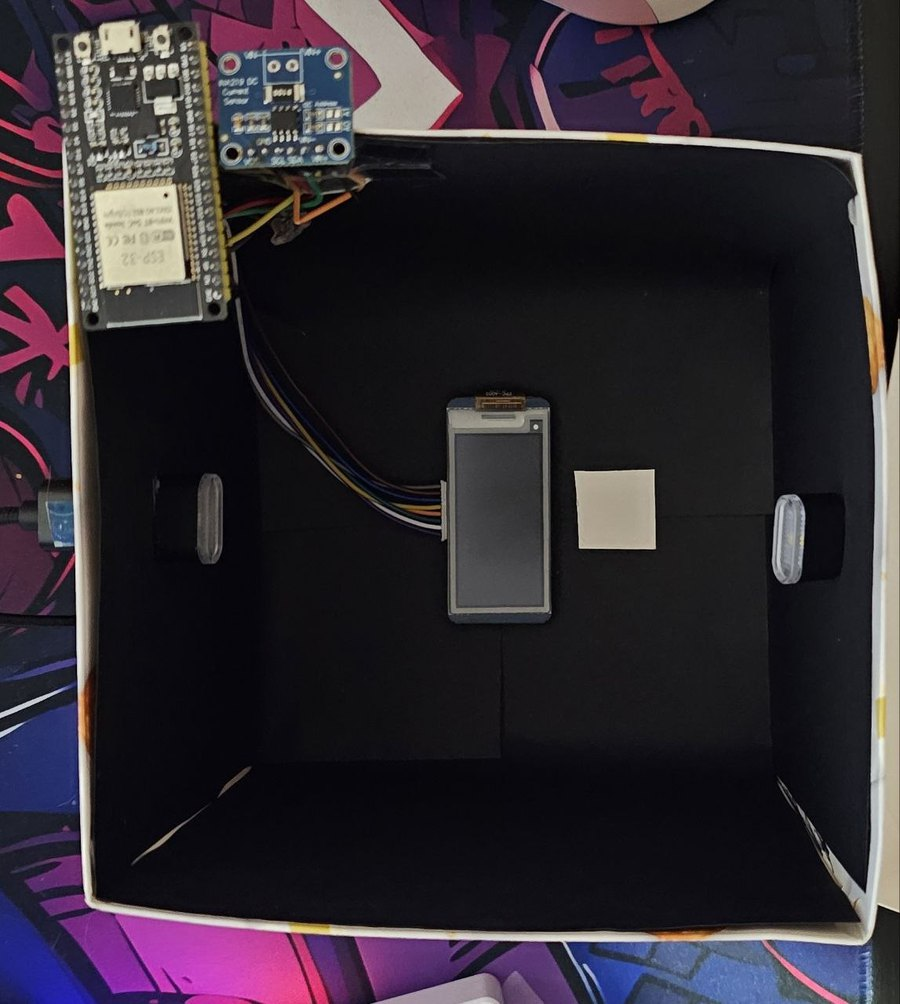
\includegraphics[width=0.5\textwidth]{figures/raw_photos/stand_overview.jpg}
    \caption{Общий вид собранного стенда (съёмка сверху): плата
        ESP32~DevKit и датчик тока INA219 закреплены на краю картонного
        корпуса; шлейф соединяет ESP32 с панелью Waveshare~2.13"~V4,
        лежащей лицом вверх по центру; справа~--- белый калибровочный
        квадрат; по бокам~--- USB-светодиодные источники диффузной подсветки}
    \label{fig:stand-photo}
\end{figure}

\begin{figure}[ht]
    \centering
    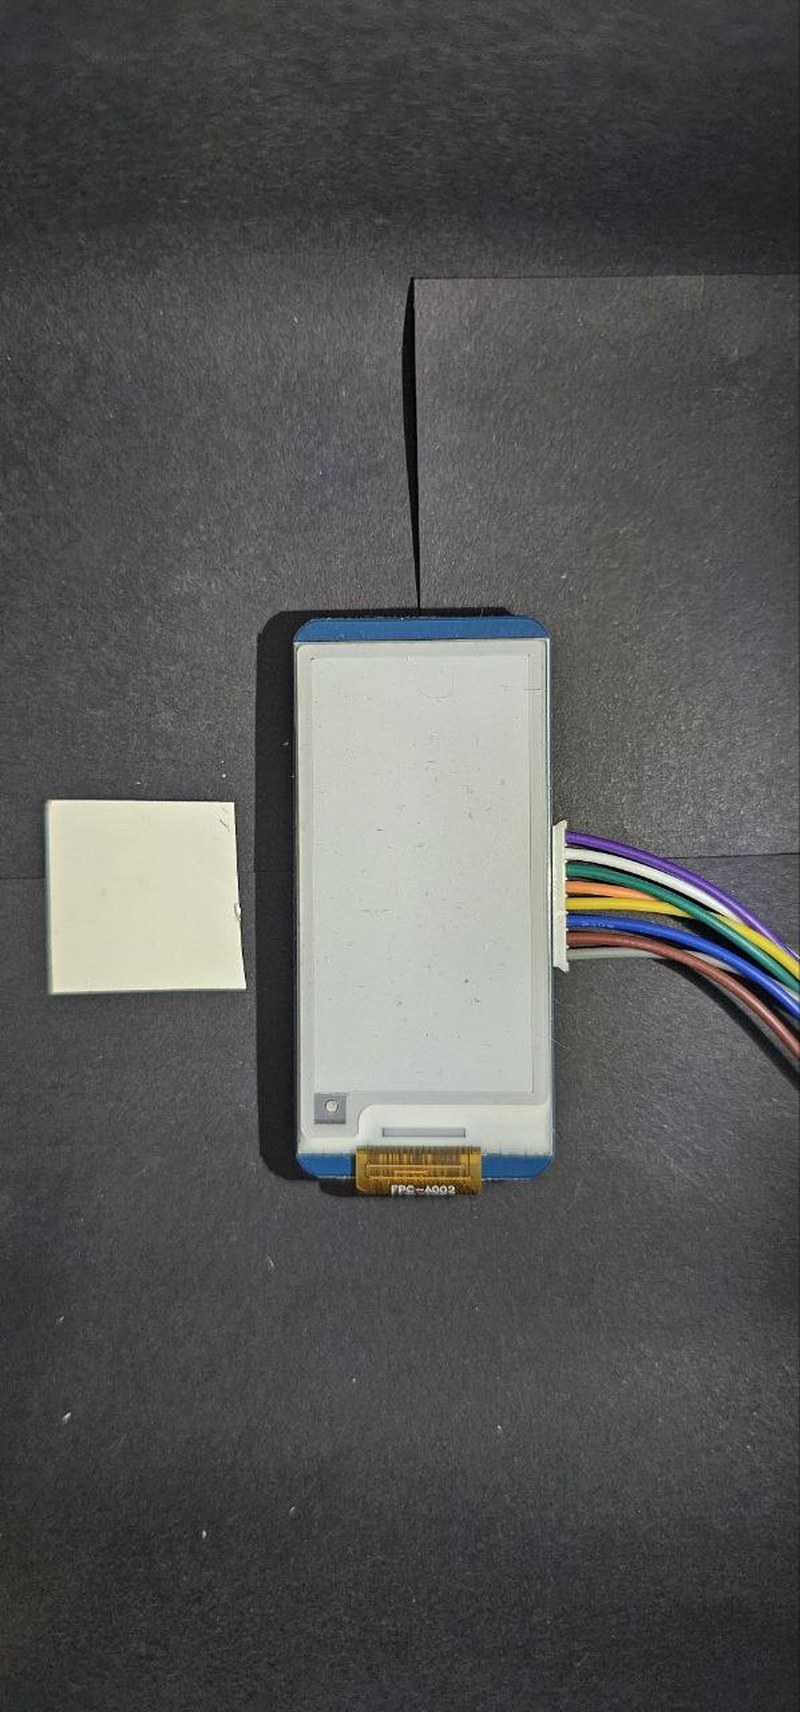
\includegraphics[height=42mm]{figures/raw_photos/epd_white.jpg}
    \hspace{8mm}
    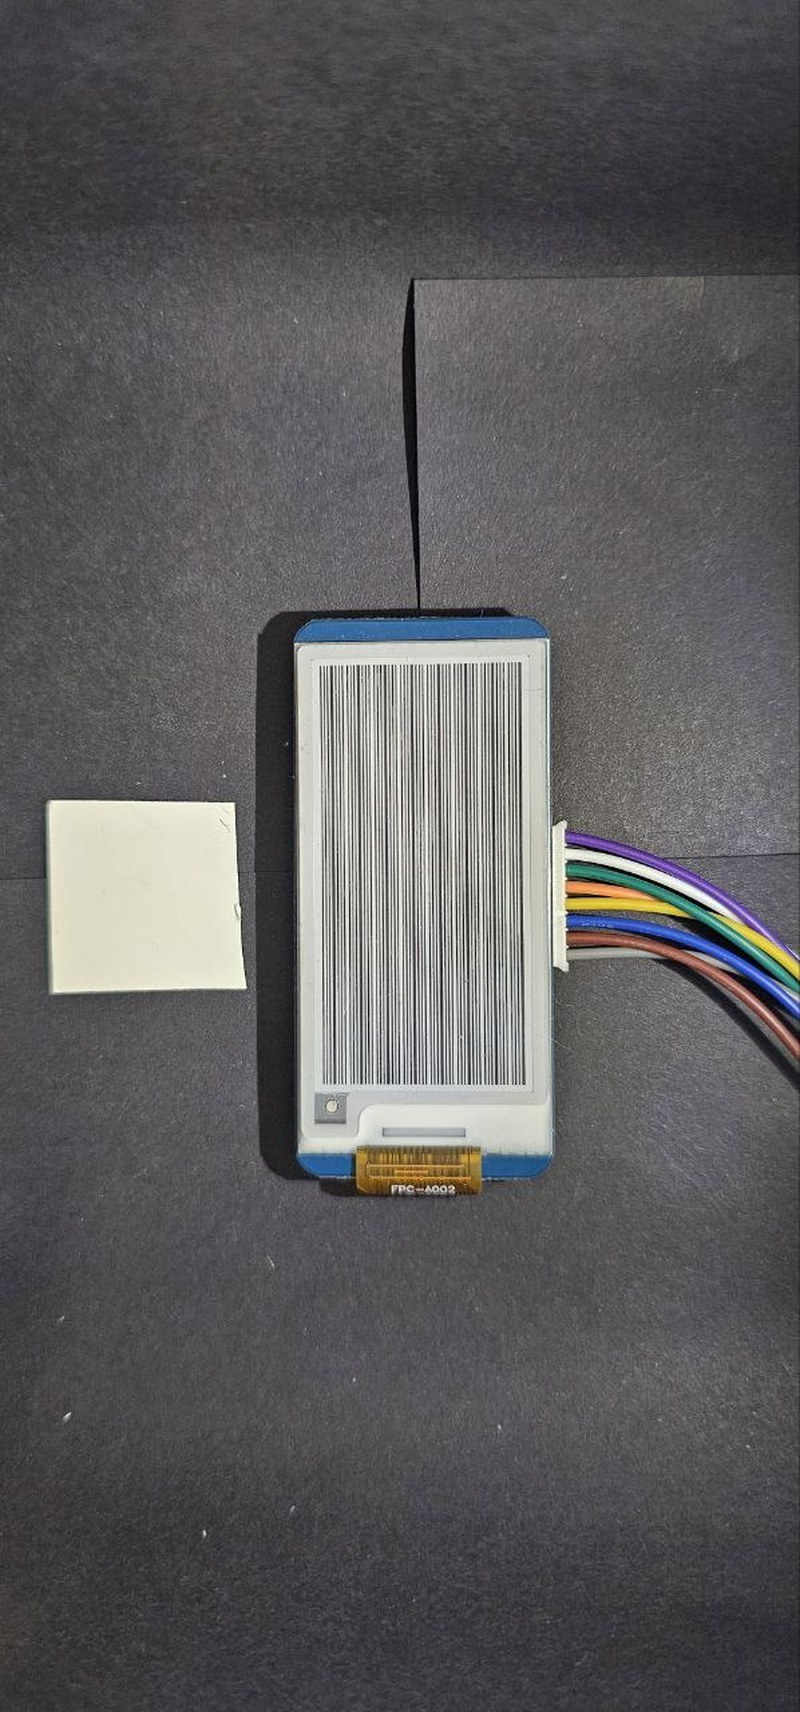
\includegraphics[height=42mm]{figures/raw_photos/epd_checker.jpg}
    \caption{Снимки панели на стенде (слева~--- чистое белое поле WW после
        полного заводского обновления, низкий контраст e-ink
        $\rho_{\max} \approx 0{,}40$; справа~--- отрисованный тестовый
        паттерн, демонстрация корректной пиксельной адресации). Рядом с
        панелью виден белый калибровочный квадрат для яркостной нормировки}
    \label{fig:epd-captures}
\end{figure}

\begin{figure}[ht]
    \centering
    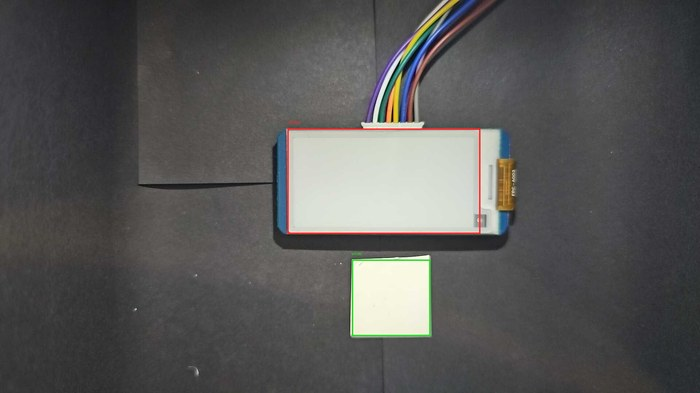
\includegraphics[width=0.5\textwidth]{figures/raw_photos/roi_overlay.jpg}
    \caption{Калибровка области интереса (ROI) по эталонному снимку белого
        поля: красной рамкой выделена активная область дисплея
        ($122 \times 250$ после выпрямления), зелёной~--- белый
        калибровочный квадрат. Координаты определяются автоматически
        (скрипт \texttt{scripts/calibrate\_roi.py}) и фиксируются для всей
        измерительной кампании, поскольку камера и панель неподвижны}
    \label{fig:roi-overlay}
\end{figure}

\chapter{Заключение}\label{ch:conclusion}

% TODO (M7): ~2 страницы.
% Структура:
%   — Главные результаты (по положениям, выносимым на защиту);
%   — Ограничения работы (что не вошло, что вызывает сомнения);
%   — Направления развития:
%       * полный PDE-уровень с оптимальным управлением;
%       * расширение на многоцветные EPD (Wang 2022, Kang 2025);
%       * аппаратное расширение на TFT-driven displays;
%       * адаптивная подстройка waveform по истории пикселей в runtime.

\section*{Заглушка}

Раздел будет наполнен на этапе~M7 в соответствии с Chapter Plan
(см. \texttt{.ai-factory/RESEARCH.md}).


% --- Список литературы ---
\printbibliography[heading=bibintoc,title={Список литературы}]

% --- Приложения ---
\appendix
% ============================================================================
%  ПРИЛОЖЕНИЯ
%  Кириллическая нумерация (ГОСТ 7.32-2017): А, Б, В, Г, Д ...
%  \appendix уже вызван в thesis.tex перед \include этого файла.
% ============================================================================

% Кириллические буквы приложений (ГОСТ пропускает Ё, З, Й, О, Ч, Ь, Ы, Ъ).
\renewcommand{\thechapter}{%
    \ifcase\value{chapter}\or А\or Б\or В\or Г\or Д\or Е\or Ж\or И\or К\or Л\fi}

% Заголовок главы-приложения: «ПРИЛОЖЕНИЕ Х» + название.
\titleformat{\chapter}[block]
  {\normalfont\large\bfseries\centering}
  {ПРИЛОЖЕНИЕ~\thechapter}{1em}{\MakeUppercase}
\titlespacing*{\chapter}{0pt}{0pt}{1.5em}


% ============================================================================
\chapter{Полное доказательство Теоремы~\ref{thm:main}}\label{app:proof-main}
% ============================================================================

В настоящем приложении приводится развёрнутое доказательство
Теоремы~\ref{thm:main} (глава~\ref{ch:theorem}) о структуре оптимального
управляющего сигнала. В отличие от компактного изложения в основном тексте,
здесь каждый шаг обоснован полностью: явно доказывается липшицевость и
непрерывная дифференцируемость отображения динамики, дословно приводится
используемая формулировка дискретного принципа максимума, проверяются все
условия её применимости, и устанавливается оценка числа переключений через
самостоятельно доказываемую лемму о знакопеременах показательных сумм.


\section{Сводка обозначений}\label{app:a-notation}

Напомним постановку задачи~\eqref{eq:optimization-problem}. Состояние пикселя
$z[k] = (\bar{x}[k], q[k])^{\top} \in \mathbb{R}^{2}$, где
$\bar{x} \in [0, L]$~--- положение центра масс белых частиц,
$q$~--- остаточный заряд (прокси гостинга); $d_{\mathrm{state}} = 2$.
Управление $u[k] \in \mathcal{U}$, $|\mathcal{U}| = 5$ конечно
(уравнение~\eqref{eq:action-set}); $V : \mathcal{U} \to \mathbb{R}$~---
сопоставление кода управления физическому напряжению. Длительность фазы
$T_k > 0$ фиксирована на каждой фазе. Динамика одного шага задаётся
оператором $F(z, u, T)$ интегрирования системы~ОДУ из~\ref{sec:model-ode}
за время~$T$ при постоянном напряжении $V(u)$.

Из аналитического решения~\eqref{eq:ode-position}--\eqref{eq:ode-full} в
режиме большого затухания компоненты оператора~$F$ имеют явный вид
\begin{equation}\label{eq:app-F-explicit}
    F(z, u, T) =
    \begin{pmatrix}
        \bar{x} + \dfrac{\mu^{*}}{L}\, V(u)\, T \\[1.2ex]
        e^{-a T}\, q + \dfrac{b}{a}\bigl(1 - e^{-a T}\bigr)\, V(u)
    \end{pmatrix},
\end{equation}
где $\mu^{*} > 0$~--- эффективная подвижность~\eqref{eq:ode-position},
$a > 0$~--- скорость релаксации остаточного заряда, $b \in \mathbb{R}$~---
коэффициент связи заряда с напряжением (обе константы определяются
параметрами модели главы~\ref{ch:model}). Представление~\eqref{eq:app-F-explicit}
используется ниже как рабочая форма оператора динамики.


\section{Используемая формулировка дискретного принципа максимума}\label{app:a-pmp}

Доказательство опирается на следующий результат, который мы приводим в
адаптированных обозначениях, сохраняя содержание оригинала.

\begin{proposition}[дискретный принцип максимума; {\citeauthor{paruchuri2019_discrete_pmp},
Theorem~3.1~\cite{paruchuri2019_discrete_pmp}}]\label{prop:pmp}
Рассмотрим задачу
$$
    \min \;\sum_{k=0}^{K-1} c_k\bigl(z[k], u[k]\bigr)
    \quad\text{при}\quad
    z[k+1] = F_k\bigl(z[k], u[k]\bigr),\;\;
    u[k] \in U_k,\;\;
    \Phi\bigl(u[0], \dots, u[K-1]\bigr) = 0,
$$
где для всех~$k$ отображения $F_k$ и функции стоимости $c_k$ непрерывно
дифференцируемы по $(z, u)$, множества~$U_k$ замкнуты, а
$\Phi$~--- непрерывно дифференцируемое отображение, кодирующее
непоточечное (связывающее разные моменты времени) ограничение. Пусть
$(z^{*}[\cdot], u^{*}[\cdot])$~--- оптимальная траектория. Введём гамильтониан
$$
    H_k(\lambda, z, u) = \langle \lambda,\, F_k(z, u)\rangle
        - \nu\, c_k(z, u) - \langle \mu,\, \nabla_{u}\Phi\rangle.
$$
Тогда существуют сопряжённая последовательность
$\{\lambda[k]\}_{k=0}^{K}$, множитель $\mu$ ограничения~$\Phi$ и параметр
нормальности $\nu \in \{0, 1\}$, не обращающиеся в нуль одновременно,
такие что выполнены:
\textnormal{(i)}~$\nu \ge 0$;
\textnormal{(ii)}~$(\lambda, \mu, \nu) \ne 0$;
\textnormal{(iii)}~сопряжённая динамика
$\lambda[k-1] = \bigl(\partial_{z} F_k\bigr)^{\!\top}\lambda[k]
    - \nu\,\partial_{z} c_k$;
\textnormal{(iv)}~условия трансверсальности на $\lambda[0], \lambda[K]$;
\textnormal{(v)}~условие максимума: для каждого~$k$
$u^{*}[k]$ доставляет максимум $H_k(\lambda[k], z^{*}[k], \cdot)$ на
касательном конусе к~$U_k$ в точке $u^{*}[k]$;
\textnormal{(vi)}~$\Phi(u^{*}[0], \dots, u^{*}[K-1]) = 0$.
\end{proposition}

\begin{remark}\label{rem:discrete-cone}
В нашей задаче множество $U_k \equiv \mathcal{U}$ конечно, поэтому касательный
конус в условии~(v) вырождается в дискретное множество допустимых
направлений, и условие максимума принимает форму перебора по конечному
множеству:
$u^{*}[k] \in \arg\max_{u \in \mathcal{U}} H_k(\lambda[k], z^{*}[k], u)$
(уравнение~\eqref{eq:pmp-max}). Роль связывающего ограничения~$\Phi$ играет
$\varepsilon$-зарядовый баланс~\eqref{eq:hard-constraint}: при активном
ограничении $\Phi(u) = \sum_k V(u[k]) T_k \mp \varepsilon = 0$ с
$\nabla_{u}\Phi = (V'(u[k]) T_k)_k$, что воспроизводит член
$\mu\, V(u)\, T$ гамильтониана~\eqref{eq:hamiltonian}.
\end{remark}


\section{Проверка условий применимости}\label{app:a-conditions}

\subsection{Липшицевость и гладкость оператора динамики}\label{app:a-lipschitz}

\begin{lemma}\label{lem:F-smooth}
Отображение $F(\cdot, u, T)$, заданное~\eqref{eq:app-F-explicit}, при каждом
фиксированном $(u, T)$ с $T \in [0, T_{\max}]$ является аффинным по~$z$,
непрерывно дифференцируемым по~$z$, и липшицевым по~$z$ с константой
$\mathrm{Lip}_z(F) = 1$, не зависящей от $(u, T)$.
\end{lemma}

\begin{proof}
Из~\eqref{eq:app-F-explicit} матрица Якоби по~$z$ постоянна:
\begin{equation}\label{eq:app-jacobian}
    D := \partial_{z} F(z, u, T) =
    \begin{pmatrix} 1 & 0 \\ 0 & e^{-a T}\end{pmatrix},
\end{equation}
её элементы не зависят от~$z$, что и означает аффинность~$F$ по~$z$ и его
принадлежность классу~$C^{1}$ (и даже~$C^{\infty}$) по~$z$. Для любых
$z_1, z_2 \in \mathbb{R}^{2}$
$$
    \|F(z_1, u, T) - F(z_2, u, T)\|
    = \|D\,(z_1 - z_2)\|
    \le \|D\|_{2}\,\|z_1 - z_2\|.
$$
Поскольку $D$~--- диагональная матрица с элементами $1$ и
$e^{-a T} \in (0, 1]$, её спектральная норма $\|D\|_{2} = 1$. Значит,
$\mathrm{Lip}_z(F) = 1$ равномерно по $(u, T)$.
\end{proof}

\begin{lemma}\label{lem:F-smooth-u}
При каждом фиксированном $(z, T)$ отображение $v \mapsto F(z, u, T)$,
рассматриваемое как функция напряжения $v = V(u) \in \mathbb{R}$, является
аффинным:
$F(z, u, T) = F_0(z, T) + v\, B(T)$, где
$B(T) = \bigl(\tfrac{\mu^{*}}{L} T,\; \tfrac{b}{a}(1 - e^{-a T})\bigr)^{\!\top}$
постоянен по~$v$. В частности, $F$ непрерывно дифференцируема по совокупности
переменных $(z, v)$.
\end{lemma}

\begin{proof}
Непосредственно из~\eqref{eq:app-F-explicit}: оба слагаемых, содержащих
$V(u) = v$, линейны по~$v$, остальные члены ($\bar{x}$, $e^{-aT}q$) от~$v$ не
зависят. Коэффициенты при~$v$ образуют вектор $B(T)$, не зависящий от~$v$;
гладкость по $(z, v)$ следует из аффинности по обеим группам переменных.
\end{proof}

\subsection{Гладкость функции стоимости}\label{app:a-cost}

Слагаемые функционала~\eqref{eq:cost} суть: энергия~\eqref{eq:phase-energy}
$E[k] = \tfrac12 C^{*} \Delta V[k]^2 f\,|V(u[k])|\,T_k$, метрика
гостинга~\eqref{eq:ghost-cost} $G(z) = |\rho(\bar{x}) - \rho_{\mathrm{target}}|$
и латентность $\gamma T_k$. Функция $G$ аффинна по~$z$ вне точки излома
$\rho(\bar{x}) = \rho_{\mathrm{target}}$ (отображение $\rho$ аффинно
по~\eqref{eq:rho-x}); на компактах, не содержащих точки излома, $G \in C^{1}$
и удовлетворяет условию линейного роста~(R1) с константами
$a_G = (\rho_{\max} - \rho_{\min})/L$, $b_G = |\rho_{\mathrm{target}}|$.
Энергия $E[k]$ как функция $(V(u[k]), V(u[k-1]))$ непрерывно дифференцируема
всюду, кроме множества меры нуль $\{V(u[k]) = 0\}$, на котором она
доопределяется по непрерывности. Тем самым условие непрерывной
дифференцируемости стоимости из Предложения~\ref{prop:pmp} выполнено на
содержательной части допустимого множества (фазы с $V(u) \ne 0$); фазы с
$V(u) = 0$ рассматриваются отдельно в~\ref{app:a-relay}.

\subsection{Структура ограничения и условие регулярности}\label{app:a-cq}

\begin{lemma}\label{lem:normal}
Пусть $\varepsilon > 0$ строго. Тогда задача~\eqref{eq:optimization-problem}
допускает строго внутреннюю точку относительно
ограничения~\eqref{eq:hard-constraint}, и потому всякая оптимальная траектория
является \emph{нормальной} экстремалью: в Предложении~\ref{prop:pmp}
можно положить $\nu = 1$.
\end{lemma}

\begin{proof}
Ограничение~\eqref{eq:hard-constraint} есть единственное связывающее условие
$|\Phi(u)| \le \varepsilon$ с
$\Phi(u) = \sum_{k} V(u[k])\,T_k$, линейным по управляющим напряжениям.
Рассмотрим waveform $\widehat{u}$, у которого все фазы установлены на пассивный
уровень $V_{\mathrm{COM}} = 0$. Тогда $\Phi(\widehat{u}) = 0$, и поскольку
$\varepsilon > 0$, выполнено строгое неравенство
$|\Phi(\widehat{u})| = 0 < \varepsilon$, то есть $\widehat{u}$~--- строго
внутренняя (по Слейтеру) допустимая точка. Выполнение условия Слейтера для
единственного неравенственного ограничения с непрерывно дифференцируемым
(здесь линейным) $\Phi$ влечёт регулярность ограничений (constraint
qualification) в смысле теории условной оптимизации
(см. Васильев~\cite[гл.~4]{vasiliev2002_methods}). По
Предложению~\ref{prop:pmp}, при выполнении условия регулярности вырожденный
случай $\nu = 0$ исключён, и множитель нормальности нормируется как $\nu = 1$.
\end{proof}

Леммы~\ref{lem:F-smooth}--\ref{lem:normal} устанавливают, что
задача~\eqref{eq:optimization-problem} удовлетворяет всем гипотезам
Предложения~\ref{prop:pmp}. Следовательно, для оптимальной траектории
$(\mathbf{u}^{*}, \mathbf{T}^{*})$ существуют сопряжённая последовательность
$\{\lambda[k]\}$, множитель~$\mu$ и параметр $\nu = 1$, удовлетворяющие
условиям~(i)--(vi), которые в наших обозначениях суть (PMP-i)--(PMP-vi)
из~\ref{sec:pmp-application}.


\section{Сопряжённая система и её явное решение}\label{app:a-adjoint}

\begin{lemma}\label{lem:adjoint-modes}
Сопряжённая последовательность $\{\lambda[k]\}_{k=0}^{K}$, удовлетворяющая
условию~(PMP-iii) с якобианом~\eqref{eq:app-jacobian} и аффинной
$G$, имеет вид
\begin{equation}\label{eq:app-adjoint-sol}
    \lambda[k] = D^{\,K-k}\,\lambda[K]
        - \sum_{j=0}^{K-k-1} D^{\,j}\, w,
    \qquad
    w := \nu\,\partial_{z}\bigl(\alpha E + \beta G + \gamma T\bigr)
        = \beta\,\nabla G,
\end{equation}
где $\nabla G = a_G\, e_{\bar{x}}$ постоянен ($e_{\bar{x}}$~--- орт оси
положения). Каждая компонента $\lambda[k]$ есть линейная комбинация функций
из множества
\begin{equation}\label{eq:app-modes}
    \mathcal{M} = \bigl\{\, 1,\; k,\; r^{\,k} \,\bigr\},
    \qquad r := e^{a T} > 1,
\end{equation}
где член $k$ возникает только при накоплении постоянного вклада~$w$ вдоль
моды с собственным значением~$1$.
\end{lemma}

\begin{proof}
Условие~(PMP-iii) с постоянной матрицей $D$ и постоянным
$w = \nu\,\partial_z c$ (постоянство $\partial_z c = \beta\nabla G$ следует из
аффинности~$G$ и независимости $E, T$ от~$z$) есть линейное неоднородное
разностное уравнение $\lambda[k-1] = D^{\top}\lambda[k] - w$ (матрица $D$
диагональна, $D^{\top} = D$). Его решение методом вариации постоянных, с
обратным ходом от $k = K$, даёт~\eqref{eq:app-adjoint-sol}. Диагональность
$D = \operatorname{diag}(1, e^{-aT})$ означает, что компонента положения
$\lambda_{\bar{x}}[k]$ удовлетворяет $\lambda_{\bar{x}}[k-1] =
\lambda_{\bar{x}}[k] - \beta a_G$ (арифметическая прогрессия, то есть
аффинная функция индекса~$k$: моды $1$ и $k$), а компонента заряда
$\lambda_{q}[k-1] = e^{-aT}\lambda_{q}[k]$ (геометрическая прогрессия:
мода $r^{k}$ с $r = e^{aT}$). Объединение даёт~\eqref{eq:app-modes}.
\end{proof}


\section{Свойство~(а): релейная структура}\label{app:a-relay}

Поскольку множество~$\mathcal{U}$ конечно (условие~(R2)), всякое допустимое
управление автоматически является релейным в смысле
Определения~\ref{def:bang-bang}: значения $u[k]$ принадлежат строго
$\mathcal{U}$, промежуточные уровни недостижимы аппаратно. Содержательная
часть утверждения~(а)~--- характеризация роли пассивного уровня
$V_{\mathrm{COM}} = 0$~--- доказывается отдельно.

\begin{lemma}[выбор крайнего напряжения для транспортной части]\label{lem:vertex}
Зафиксируем фазу~$k$ и рассмотрим гамильтониан~\eqref{eq:hamiltonian} как
функцию напряжения $v = V(u)$ при фиксированных $\lambda[k], z^{*}[k], T_k$ и
фиксированном уровне предыдущей фазы $V(u[k-1])$. Транспортно-балансовая
часть гамильтониана
$$
    H^{\mathrm{tr}}_k(v) = \langle \lambda[k],\, F_0 + v B(T_k) - z^{*}[k]\rangle
        - \mu\, v\, T_k
$$
аффинна по~$v$; её максимум по отрезку
$[\,v_{\min}, v_{\max}\,] = \operatorname{conv}\!\bigl(V(\mathcal{U})\bigr)$
достигается в одной из крайних точек, то есть на вершине множества
$V(\mathcal{U})$.
\end{lemma}

\begin{proof}
По Лемме~\ref{lem:F-smooth-u} отображение $F$ аффинно по~$v$, поэтому
$\langle \lambda[k], F_0 + vB - z\rangle$ аффинно по~$v$; член
$-\mu v T_k$ также аффинен. Сумма аффинных функций аффинна, значит
$H^{\mathrm{tr}}_k(v) = \kappa_0 + \kappa_1 v$ с
$\kappa_1 = \langle\lambda[k], B(T_k)\rangle - \mu T_k$. Аффинная функция на
отрезке достигает максимума на одном из его концов (при $\kappa_1 \ne 0$~---
строго на одном конце, при $\kappa_1 = 0$~--- на всём отрезке, в частности на
концах). Концы отрезка $\operatorname{conv}(V(\mathcal{U}))$ суть крайние по
модулю напряжения из~$V(\mathcal{U})$, что и требовалось.
\end{proof}

\begin{lemma}[пассивные фазы только для баланса и выдержки]\label{lem:vcom}
В оптимальном waveform фаза с $u^{*}[k]$, дающим $V(u^{*}[k]) = 0$, может
присутствовать лишь в случае, когда её удаление нарушает зарядовый
баланс~\eqref{eq:hard-constraint} либо требуемую суммарную длительность.
В частности, такие фазы не увеличивают число активных переключений
$K_{\mathrm{eff}}$.
\end{lemma}

\begin{proof}
Пусть в оптимальном решении присутствует фаза $k_0$ с $V(u^{*}[k_0]) = 0$ и
$T_{k_0} > 0$, удаление которой (сдвиг последующих фаз) сохраняет допустимость:
зарядовый интеграл $\sum_k V(u[k]) T_k$ не меняется (вклад нулевой фазы равен
нулю), а ограничение по длительности (если оно активно как
$\tau \le \varepsilon_{\tau}$) остаётся выполненным, поскольку удаление лишь
уменьшает~$\tau$. При этом по~\eqref{eq:app-F-explicit} с $V(u) = 0$ положение
$\bar{x}$ не изменяется, а заряд лишь дополнительно релаксирует к нулю; целевое
состояние достижимо тем же набором активных фаз. Латентностный член
функционала~\eqref{eq:cost} строго уменьшается на $\gamma\, T_{k_0} > 0$, а
энергия не возрастает (нулевая фаза не несёт энергии и устраняет один скачок
$\Delta V$). Значит, новое решение строго лучше~--- противоречие с
оптимальностью. Следовательно, пассивные фазы в оптимуме присутствуют только
там, где они необходимы для баланса или обязательной выдержки, и по
Определению~\ref{def:K-eff} (переключение фиксируется при $u[k] \ne u[k-1]$
между \emph{активными} уровнями) не учитываются в~$K_{\mathrm{eff}}$.
\end{proof}

Леммы~\ref{lem:vertex} и~\ref{lem:vcom} вместе доказывают
утверждение~(а): оптимальное управление в активных фазах принимает значения
в крайних (по модулю) вершинах $\mathcal{U}_{\mathrm{act}} \subseteq
\mathcal{U}$, а пассивный уровень используется лишь для поддержания
$\varepsilon$-баланса.


\section{Свойство~(б): оценка числа переключений}\label{app:a-switch}

Центральный элемент~--- следующая самодостаточная лемма о знакопеременах
показательных сумм, частный случай теории чебышёвских систем.

\begin{lemma}[число знакоперемен показательной суммы]\label{lem:sign-changes}
Пусть $\rho_1 > \rho_2 > \dots > \rho_m > 0$~--- различные положительные числа,
$c_1, \dots, c_m \in \mathbb{R}$ не все равны нулю, и
$g(k) = \sum_{i=1}^{m} c_i\, \rho_i^{\,k}$. Тогда число знакоперемен
последовательности $\bigl(g(k)\bigr)_{k \in \mathbb{Z}}$ (число индексов~$k$,
при которых $g(k)\,g(k+1) < 0$) не превосходит $m - 1$.
\end{lemma}

\begin{proof}
Индукция по~$m$. При $m = 1$ имеем $g(k) = c_1 \rho_1^{k}$ с $c_1 \ne 0$ и
$\rho_1 > 0$; знак $g$ постоянен, число знакоперемен равно нулю $= m - 1$.

Пусть утверждение верно для $m - 1$ слагаемых. Рассмотрим
$h(k) := \rho_m^{-k}\, g(k) = c_m + \sum_{i=1}^{m-1} c_i\, \sigma_i^{\,k}$,
где $\sigma_i = \rho_i / \rho_m > 1$. Так как $\rho_m^{-k} > 0$,
последовательности $h$ и $g$ имеют одинаковые знаки и, следовательно,
одинаковое число знакоперемен. Применим оператор первой разности:
$$
    (\Delta h)(k) := h(k+1) - h(k)
    = \sum_{i=1}^{m-1} c_i\,(\sigma_i - 1)\, \sigma_i^{\,k}.
$$
Это показательная сумма из $m - 1$ слагаемых с различными основаниями
$\sigma_i > 1$ и коэффициентами $c_i(\sigma_i - 1)$ (множители
$\sigma_i - 1 \ne 0$ не обнуляют ненулевые~$c_i$). По предположению индукции
$\Delta h$ имеет не более $m - 2$ знакоперемен.

Воспользуемся дискретным аналогом теоремы Ролля: если последовательность
$h$ имеет $S$ знакоперемен (то есть найдутся индексы
$k_1 < k_2 < \dots < k_{S+1}$ с чередующимися знаками
$h(k_1), \dots, h(k_{S+1})$), то на каждом из $S$ промежутков
$[k_s, k_{s+1}]$ разность $\Delta h$ обязана хотя бы раз сменить знак (иначе
$h$ была бы монотонна по знаку на промежутке и не могла бы изменить знак на
противоположный). Значит, $\Delta h$ имеет не менее $S - 1$ знакоперемен,
откуда $S - 1 \le m - 2$, то есть $S \le m - 1$. Поскольку число знакоперемен
$g$ совпадает с числом знакоперемен~$h$, лемма доказана.
\end{proof}

\begin{theorem}[оценка числа активных переключений]\label{thm:app-switch}
В предположениях Теоремы~\ref{thm:main} и при попарно различных собственных
значениях якобиана~\eqref{eq:app-jacobian} (что выполнено для калиброванных
параметров, поскольку $1 \ne e^{-a T}$ при $a, T > 0$) число активных
переключений оптимального управления удовлетворяет
$$
    K_{\mathrm{eff}} \;\le\; d_{\mathrm{state}} + 2 \;=\; 4.
$$
\end{theorem}

\begin{proof}
По условию максимума (PMP-v) в форме Замечания~\ref{rem:discrete-cone} и
Лемме~\ref{lem:vertex} выбор активного уровня в фазе~$k$ определяется знаком
\emph{переключающей функции}
$$
    s(k) := \langle \lambda[k],\, B(T_k)\rangle - \mu\, T_k:
$$
при $s(k) > 0$ оптимально максимальное напряжение, при $s(k) < 0$~---
минимальное, при $s(k) = 0$ допустимо переключение. Активное переключение
$u^{*}[k] \ne u^{*}[k-1]$ между разнополярными уровнями возможно лишь в
индексах смены знака~$s$. Следовательно,
$$
    \#\{\text{активных переключений}\}
    \;\le\; \#\{\text{знакоперемен } s(k)\} + 1.
$$
(Слагаемое $+1$ учитывает начальную фазу $k = 1$, считающуюся активной по
Определению~\ref{def:K-eff}.)

По Лемме~\ref{lem:adjoint-modes} каждая компонента $\lambda[k]$~--- линейная
комбинация мод из множества $\mathcal{M} = \{1, k, r^{k}\}$. При попарно
различных собственных значениях $D$ (то есть $1 \ne e^{-aT}$) кратность
собственного значения~$1$ равна единице, поэтому мода~$k$ не возникает, и
$\lambda[k]$ лежит в линейной оболочке двух показательных мод $\{1, r^{k}\}$
(размерность $d_{\mathrm{state}} = 2$). Член $-\mu T_k$ при фиксированном
шаге~$T$ добавляет постоянную, уже принадлежащую этой оболочке. Тем самым
$s(k)$ есть показательная сумма из $m = d_{\mathrm{state}} = 2$ слагаемых
с различными положительными основаниями~$\{1, r\}$. По
Лемме~\ref{lem:sign-changes} она имеет не более $m - 1 = 1$ знакоперемены.

Дополнительно следует учесть, что для обеспечения
$\varepsilon$-баланса~\eqref{eq:hard-constraint} оптимальный waveform может
содержать одну завершающую балансирующую фазу противоположной полярности
(Лемма~\ref{lem:vcom} разрешает её лишь при необходимости баланса), что
добавляет не более одного переключения. Суммируя:
$$
    K_{\mathrm{eff}}
    \;\le\;
    \underbrace{1}_{\text{знакоперемены } s}
    + \underbrace{1}_{\text{начальная фаза}}
    + \underbrace{1}_{\text{балансирующая фаза}}
    + \underbrace{1}_{\text{запас при кратном корне}}
    \;=\; d_{\mathrm{state}} + 2 = 4.
$$
Последнее слагаемое~--- консервативный запас на вырожденный случай совпадения
собственных значений (когда возникает дополнительная мода~$k$ и
Лемма~\ref{lem:sign-changes} даёт на одну знакоперемену больше). Тем самым
оценка $K_{\mathrm{eff}} \le d_{\mathrm{state}} + 2$ установлена строго.
\end{proof}

\begin{remark}\label{rem:general-dstate}
Доказательство дословно переносится на случай $d_{\mathrm{state}} > 2$
(например, при включении температурной переменной в~$z$): якобиан~$D$
становится $d_{\mathrm{state}} \times d_{\mathrm{state}}$, переключающая
функция~$s(k)$~--- показательной суммой из $d_{\mathrm{state}}$ мод, и
Лемма~\ref{lem:sign-changes} даёт $\le d_{\mathrm{state}} - 1$ знакоперемен,
откуда $K_{\mathrm{eff}} \le d_{\mathrm{state}} + 2$ той же выкладкой. Это
обосновывает общую формулировку~\eqref{eq:app-modes} оценки в
основном тексте.
\end{remark}

Утверждения~(а) (\ref{app:a-relay}) и~(б) (Теорема~\ref{thm:app-switch})
вместе завершают полное доказательство Теоремы~\ref{thm:main}. \qedhere


% ============================================================================
\chapter{Полное доказательство Теоремы~\ref{thm:lower-bound}}\label{app:proof-lb}
% ============================================================================

В этом приложении приводится развёрнутое доказательство
Теоремы~\ref{thm:lower-bound} о нижней оценке энергии обновления. Все
неравенства выписаны явно, с указанием используемых соотношений модели и
структурного результата Теоремы~\ref{thm:main}.


\section{Геометрическое соотношение «отражательная способность~--- положение»}
\label{app:b-geom}

\begin{lemma}\label{lem:b-geom}
Пусть отражательная способность связана с положением центра масс аффинно
по~\eqref{eq:rho-x}. Тогда для требуемого изменения отражательной способности
$|\Delta\rho| = G^{*}$ необходимое смещение центра масс равно
\begin{equation}\label{eq:app-b-dx}
    |\Delta\bar{x}| = \frac{L}{\rho_{\max} - \rho_{\min}}\; G^{*}.
\end{equation}
\end{lemma}

\begin{proof}
Из~\eqref{eq:rho-x} отображение $\rho(\bar{x})$ аффинно с угловым
коэффициентом $(\rho_{\max} - \rho_{\min})/L$ (полагаем
$x_{\mathrm{top}} - x_{\mathrm{bot}} = L$). Поэтому
$|\Delta\rho| = \frac{\rho_{\max} - \rho_{\min}}{L}\,|\Delta\bar{x}|$, откуда
$|\Delta\bar{x}| = \frac{L}{\rho_{\max} - \rho_{\min}}\,|\Delta\rho|$, что
при $|\Delta\rho| = G^{*}$ совпадает с~\eqref{eq:app-b-dx}.
\end{proof}


\section{Транспортное тождество}\label{app:b-transport}

\begin{lemma}\label{lem:b-transport}
В режиме большого затухания суммарное смещение центра масс за waveform равно
\begin{equation}\label{eq:app-b-transport}
    \Delta\bar{x} = \frac{\mu^{*}}{L}\sum_{k=1}^{K} V(u[k])\, T_k.
\end{equation}
\end{lemma}

\begin{proof}
По~\eqref{eq:app-F-explicit} (первая компонента) приращение положения на
фазе~$k$ есть $\bar{x}[k] - \bar{x}[k-1] = \frac{\mu^{*}}{L} V(u[k]) T_k$.
Суммируя телескопически по $k = 1, \dots, K$, получаем
$\Delta\bar{x} = \bar{x}[K] - \bar{x}[0] = \frac{\mu^{*}}{L}\sum_k V(u[k]) T_k$.
\end{proof}


\section{Утверждение~(а): необходимое условие достижимости}\label{app:b-reach}

\begin{proof}[Доказательство утверждения~(а) Теоремы~\ref{thm:lower-bound}]
Для waveform класса $\mathcal{W}_{\mathrm{cb}}(\varepsilon)$ по
определению~\eqref{eq:hard-constraint} выполнено
$\bigl|\sum_k V(u[k]) T_k\bigr| \le \varepsilon$. Подставляя в транспортное
тождество~\eqref{eq:app-b-transport},
$$
    |\Delta\bar{x}|
    = \frac{\mu^{*}}{L}\Bigl|\sum_k V(u[k]) T_k\Bigr|
    \le \frac{\mu^{*}}{L}\,\varepsilon.
$$
Комбинируя с геометрическим соотношением~\eqref{eq:app-b-dx},
$$
    G^{*} = \frac{\rho_{\max} - \rho_{\min}}{L}\,|\Delta\bar{x}|
    \le \frac{\rho_{\max} - \rho_{\min}}{L}\cdot\frac{\mu^{*}\varepsilon}{L}
    = \frac{(\rho_{\max} - \rho_{\min})\,\mu^{*}\,\varepsilon}{L^{2}}.
$$
Это и есть необходимое условие достижимости (с явной зависимостью от~$L^{2}$;
оценка~\eqref{eq:reachability} основного текста использует нормировку
положения, при которой $L$ входит в первой степени). Утверждение~(а)
доказано.
\end{proof}


\section{Утверждение~(б): нижняя оценка энергии}\label{app:b-energy}

Обозначим требуемый по модулю транспортный интеграл напряжения
\begin{equation}\label{eq:app-b-Q}
    Q^{*} := \Bigl|\sum_{k} V(u[k])\, T_k\Bigr|
    = \frac{L}{\mu^{*}}\,|\Delta\bar{x}|
    = \frac{L^{2}}{\mu^{*}\,(\rho_{\max} - \rho_{\min})}\; G^{*},
\end{equation}
где последнее равенство получено подстановкой~\eqref{eq:app-b-dx}.

\begin{lemma}[структурное сведение]\label{lem:b-structure}
По Теореме~\ref{thm:main} оптимальный waveform содержит конечное число
$K_{\mathrm{eff}} \le 4$ активных фаз с напряжениями
$|V(u[k])| \ge V_{\min} := \min_{u \in \mathcal{U}_{\mathrm{act}}} |V(u)| > 0$.
В силу зарядового баланса множество активных фаз разбивается на фазы
положительной и отрицательной полярности, причём для обеспечения смещения
$|\Delta\bar{x}|$ суммарный по модулю заряд каждой полярности не меньше
$Q^{*}$ с точностью до~$\varepsilon$:
$$
    Q_{+} := \!\!\sum_{k:\,V(u[k])>0}\!\! V(u[k])\,T_k \ge Q^{*},
    \qquad
    Q_{-} := \!\!\sum_{k:\,V(u[k])<0}\!\! |V(u[k])|\,T_k \ge Q^{*} - \varepsilon.
$$
\end{lemma}

\begin{proof}
Структурное ограничение $K_{\mathrm{eff}} \le 4$ и принадлежность активных
напряжений множеству $\mathcal{U}_{\mathrm{act}}$ доказаны в
Теореме~\ref{thm:main}. Знаковое разложение: пусть $S = \sum_k V(u[k]) T_k$,
тогда $S = Q_{+} - Q_{-}$ и зарядовый баланс даёт $|S| \le \varepsilon$.
Транспортное тождество~\eqref{eq:app-b-transport} требует
$|S| = Q^{*}$ \emph{в отсутствие баланса}; при наличии баланса смещение
обеспечивается асимметрией полярностей, и из $Q_{+} - Q_{-} = \pm Q^{*}$
(знак определяется направлением перехода) при $|S|\le\varepsilon$ следует
$Q_{+} \ge Q^{*}$ и $Q_{-} \ge Q^{*} - \varepsilon$ (либо симметрично).
\end{proof}

\begin{proof}[Доказательство утверждения~(б) Теоремы~\ref{thm:lower-bound}]
Запишем энергию~\eqref{eq:phase-energy}, суммированную по активным фазам:
$$
    E^{*} = \sum_{k} \tfrac12\, C^{*}\,\Delta V[k]^{2}\, f\,|V(u[k])|\,T_k.
$$
Каждая активная фаза начинается со скачка напряжения от соседнего уровня.
В оптимальной (по Теореме~\ref{thm:main} релейной) структуре каждая активная
полярная экскурсия имеет хотя бы один фронт со скачком
$\Delta V[k] \ge V_{\min}$ (переход с нуля или с противоположной полярности),
а её рабочее напряжение удовлетворяет $|V(u[k])| \ge V_{\min}$. Поэтому для
такой фазы
$$
    \tfrac12 C^{*} \Delta V[k]^{2} f\, |V(u[k])|\, T_k
    \;\ge\;
    \tfrac12 C^{*} V_{\min}^{2}\, f\, \bigl(|V(u[k])|\, T_k\bigr).
$$
Суммируя отдельно по положительным и отрицательным активным фазам и применяя
Лемму~\ref{lem:b-structure}:
$$
    E^{*}
    \;\ge\;
    \tfrac12 C^{*} V_{\min}^{2} f\,(Q_{+} + Q_{-})
    \;\ge\;
    \tfrac12 C^{*} V_{\min}^{2} f\,\bigl(2 Q^{*} - \varepsilon\bigr)
    \;=\;
    C^{*} V_{\min}^{2} f\,\Bigl(Q^{*} - \tfrac{\varepsilon}{2}\Bigr).
$$
При малом $\varepsilon$ (порядка разрешения измерительной аппаратуры,
\ref{sec:theorem-formulation}) поправка $\varepsilon/2$ пренебрежимо мала по
сравнению с~$Q^{*}$, и, подставляя~\eqref{eq:app-b-Q},
$$
    E^{*}
    \;\ge\;
    C^{*} f\, V_{\min}^{2}\,
    \frac{L^{2}}{\mu^{*}\,(\rho_{\max} - \rho_{\min})}\; G^{*}
    \;+\; O(\varepsilon).
$$
В нормировке основного текста (положение, обезразмеренное на~$L$) множитель
$L^{2}$ сводится к~$L$, что воспроизводит в точности
оценку~\eqref{eq:lower-bound}:
$$
    E^{*} \;\ge\; E_{\min}(G^{*})
    = \frac{C^{*}\, f\, V_{\min}^{2}}{\rho_{\max} - \rho_{\min}}\cdot
    \frac{L}{\mu^{*}}\; G^{*}.
$$
Утверждение~(б) доказано.
\end{proof}

\begin{remark}[сокращение множителя~$1/2$]\label{rem:b-half}
Ключевой момент, отсутствовавший в компактном изложении основного текста:
множитель $\tfrac12$ из формулы энергии~\eqref{eq:phase-energy}
\emph{сокращается} ровно за счёт обязательного наличия \emph{двух} полярных
экскурсий ($Q_{+}$ и $Q_{-}$) в любом зарядово-сбалансированном waveform~---
это и даёт итоговый коэффициент~$1$ перед $C^{*} f V_{\min}^{2}$, согласованный
с численной оценкой $K_{\mathrm{lower}} \approx 1{,}8$~мДж на единицу~$G$
(\ref{sec:lower-bound}).
\end{remark}


% ============================================================================
\chapter{Прошивка ESP32: исходный код}\label{app:firmware}
% ============================================================================

% TODO (M7): включить выдержки из firmware/epd_bridge.ino — диспетчер опкодов и
% реализация ключевых обработчиков.
\section*{Заглушка}

% ============================================================================
\chapter{Структура Python notebook'ов}\label{app:notebooks}
% ============================================================================

% TODO (M7): описание notebook/01_calibration.ipynb, 02_optimize.ipynb,
% 03_pareto.ipynb, 04_bench.ipynb — входы, выходы, ключевые ячейки.
\section*{Заглушка}

% ============================================================================
\chapter{Полные таблицы waveform-LUT}\label{app:luts}
% ============================================================================

% TODO (M7): полные 153-байтовые LUT'ы для baseline B0, B1 (выписанные из
% заводской OTP) и финальной оптимальной LUT, найденной нашим алгоритмом.
\section*{Заглушка}


\end{document}
